\chapter{Simulazioni}
\label{cap:simulazioni}
In questo capitolo vengono presentate in dettaglio le simulazioni effettuate in SIL e MIL. Inoltre è presente una sezione in cui verrà riportata parzialmente la soluzione per le simulazioni in PIL. Nella sezione di MIL verrà descritto il modello dei sensori e dello stimatore usato nella precedente tesi, \cite{DesTestCarm}, per il confronto. Diverse osservazioni e confronti verranno fatti tra le simulazioni. La parte finale descriverà la conclusione del lavoro e eventuali sviluppi futuri.

Nelle simulazioni verranno utilizzati i seguenti percorsi:
\begin{itemize}
		\item \textbf{STEP: } Questa sequenza di waypoint definisce una fase di decollo stazionando a 3 m dal suolo, Tabella (\ref{tab:STEP})
		\item \textbf{SQUARE: } Sequenza di decollo seguita da un percorso a 2.5 m di altezza di forma quadrata con lato di 3 m e atterraggio nell'ultima posizione, Tabella (\ref{tab:SQUARE})
		\item \textbf{BUTTERFLY: } Sequenza di decollo seguita da un percorso a croce su un area di 3 m per lato, Tabella (\ref{tab:BUTTERFLY})
		\item \textbf{SNAKE: } Sequenza di decollo fino a 2.5 m, seguita da un percorso di forma varia descritta nella Tabella (\ref{tab:SNAKE})
\end{itemize}

\section{Simulazione SIL}

\begin{figure}
	\centering
	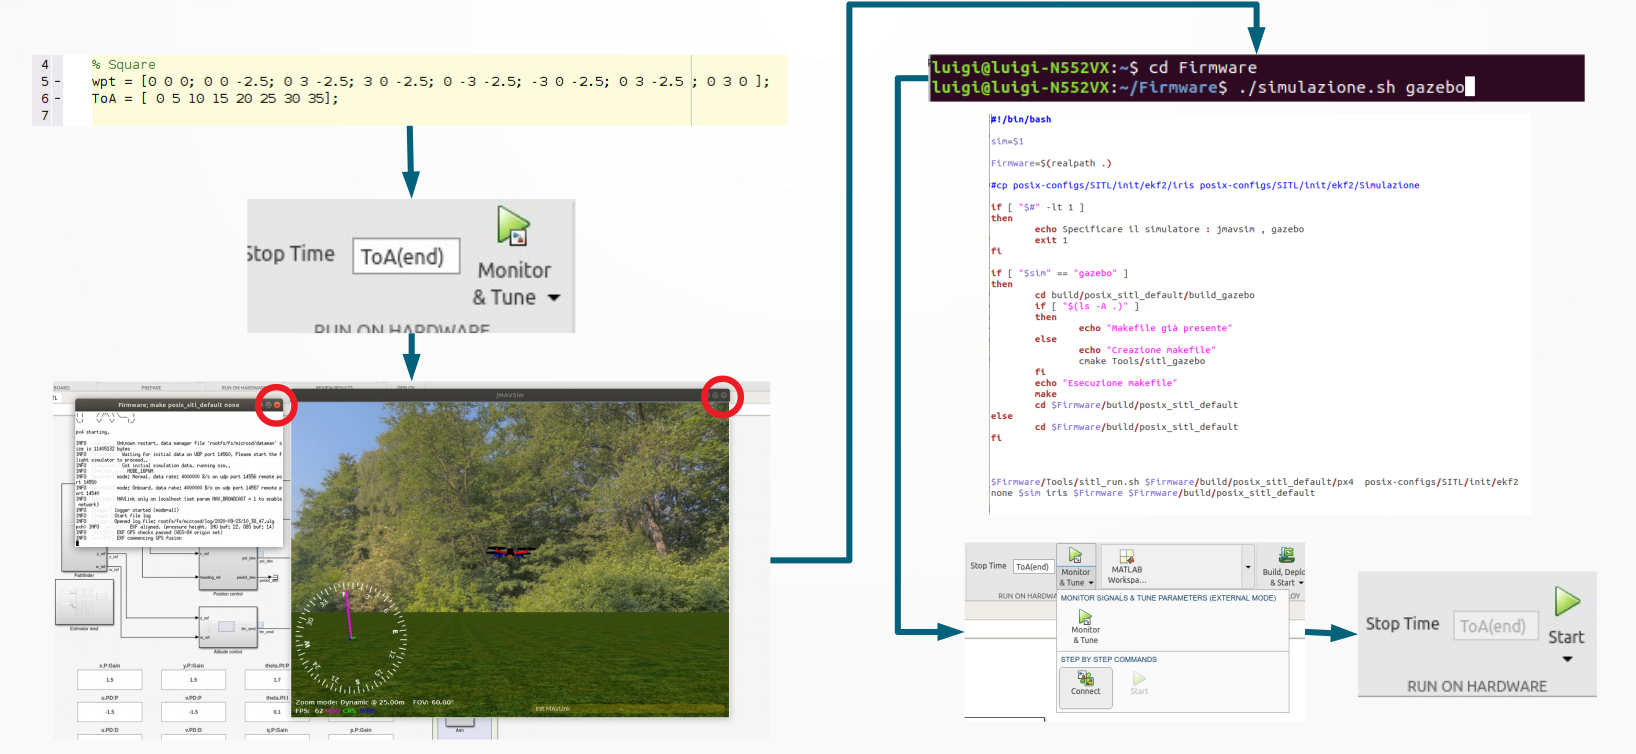
\includegraphics[width=1\textwidth]{DescrizioneAutopilota/Figure/SIMSIL}
	\caption{Descrizione del procedimento per effettuare la simulazione SIL}
	\label{fig:SIMSIL}
\end{figure}

Per effettuare la simulazione è necessaria la generazione del codice, processo che avviene in modo automatico utilizzando Simulink. Dopo aver selezionato nell'apposito file di inizializzazione la sequenza di waypoint necessari per la generazione della traiettoria, si lancia una prima fase di simulazione standard, come riportato nella guida, \cite{px4Guide}. Si termina il software lanciato dal tool, jMavSim, e attraverso la linea di comando si esegue lo script scritto appositamente per questo scopo, allegato in appendice.
Una volta avviata la simulazione e gazebo pronto, è possibile premendo il tasto "Connect", connettere i parametri presenti su Simulink con il codice generato nel software e gli strumenti necessari all'acquisizione dei dati di simulazione, e avviare il modulo di controllo. Nella Figura (\ref{fig:SIMSIL}), è riportato una descrizione grafica di questo procedimento.


\begin{table}
	\centering
	\caption{Descrizione del segnale STEP}
	\begin{tabular}{c c c c}
		\hline
		Tempo alla posizione [s] &  x [m] & y [m] & z [m]\\
		\hline
		0 & 0 & 0 & 0 \\
		3 & 0 & 0 & -3 \\
		5 & 0 & 0 & -3 \\
		\hline
	\end{tabular}	
	\label{tab:STEP}
\end{table}

\begin{table}
	\centering
	\caption{Descrizione del segnale SQUARE}
	\begin{tabular}{c c c c}
		\hline
		Tempo alla posizione [s] &  x [m] & y [m] & z [m]\\
		\hline
		0 & 0 & 0 & 0 \\
		5 & 0 & 0 & -2.5 \\
		10 & 0 & 3 & -2.5 \\
		15 & 3 & 0 & -2.5 \\
		20 & 0 & -3 & -2.5 \\
		25 & -3 & 0 & -2.5 \\
		30 & 0 & 3 & -2.5 \\
		35 & 0 & 3 & 0 \\
		\hline
	\end{tabular}	
	\label{tab:SQUARE}
\end{table}

\begin{table}
	\centering
	\caption{Descrizione del segnale BUTTERFLY}
	\begin{tabular}{c c c c}
		\hline
		Tempo alla posizione [s] &  x [m] & y [m] & z [m]\\
		\hline
		0 & 0 & 0 & 0 \\
		5 & 0 & 0 & -2.5 \\
		10 & 3 & -3 & -2.5 \\
		15 & 3 & 3 & -2.5 \\
		20 & -3 & -3 & -2.5 \\
		25 & -3 & 3 & -2.5 \\
		30 & 3 & -3 & -2.5 \\
		\hline
	\end{tabular}	
	\label{tab:BUTTERFLY}
\end{table}

\begin{table}
	\centering
	\caption{Descrizione del segnale SNAKE}
	\begin{tabular}{c c c c}
		\hline
		Tempo alla posizione [s] &  x [m] & y [m] & z [m]\\
		\hline
		0 & 0 & 0 & 0 \\
		5 & 0 & 0 & -2.5 \\
		10 & 3 & -3 & -2.5 \\
		15 & 3 & 0 & -2.5 \\
		25 & -3 & 0 & -2.5 \\
		30 & -3 & 3 & -2.5 \\
		40 & 3 & 3 & -2.5 \\
		45 &	3 & 6 & -2.5 \\
		55 & -3 & 6 & -2.5 \\
		70 & -3 & -3 & -2.5 \\
		80 & 3 & -3 & -2.5 \\
		90 & 3 & -3 & 0 \\
		\hline
	\end{tabular}	
	\label{tab:SNAKE}
\end{table}

\clearpage
\subsection{PID}

Vengono qui riportate le simulazioni SIL utilizzando la configurazione denominata PID nel capitolo \ref{cap:controllore}.

La prima simulazione riguarda il comando STEP necessario alla fase di decollo, come descritto in precedenza, utilizzando i waypoint in Tabella (\ref{tab:STEP}). Questo percorso viene eseguito generando un segnale di riferimento in velocità a profilo trapezoidale, con ampiezza massima di circa 1 m/s, leggermente raccordato in prossimità delle variazioni repentine. Il profilo di riferimento riguardante la quota risulta quindi formato da una prima parte lineare e poi costante, raccordata in prossimità dei cambiamenti di velocità. Questi segnali sono visibili di colore rosso nelle Figure (\ref{fig:STEPerrposzPID}) e (\ref{fig:STEPerrvelzPID}).
\begin{figure}
	\centering
	\begin{subfigure}{0.45\textwidth}
		\centering
		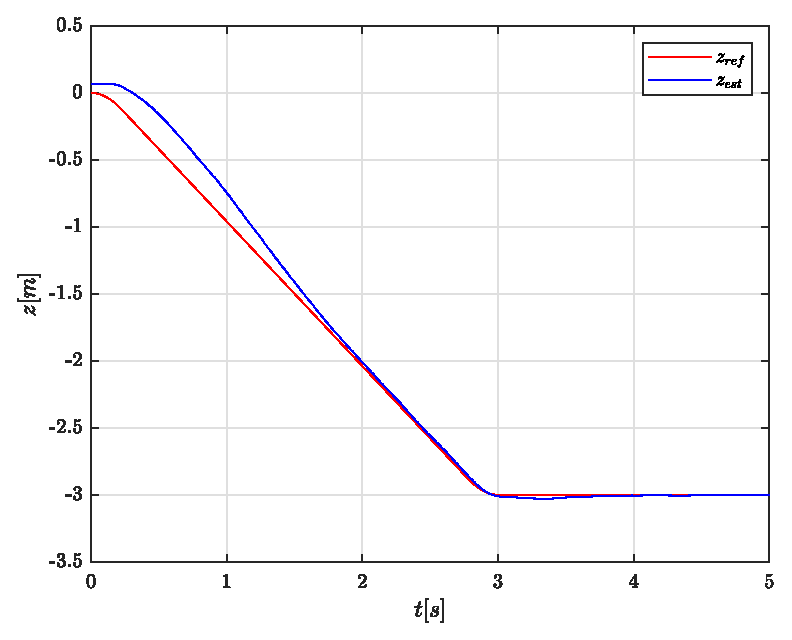
\includegraphics[width=1\textwidth]{Simulazioni/Figure/PID/STEP/AltitudeControlPos}
		\caption{Controllo posizione}
		\label{fig:STEPerrposzPID}
	\end{subfigure}
	\hfill
	\begin{subfigure}{0.45\textwidth}
		\centering
		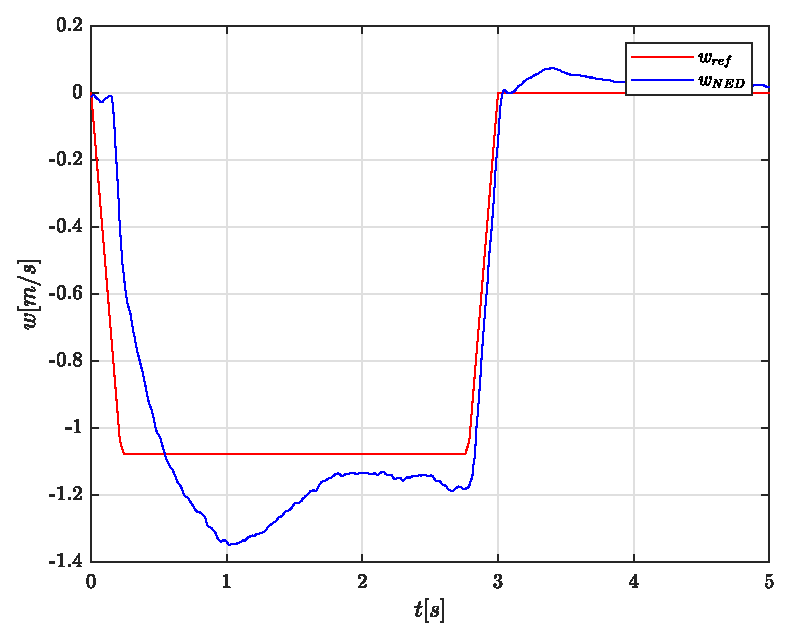
\includegraphics[width=1\textwidth]{Simulazioni/Figure/PID/STEP/AltitudeControlVel}
		\caption{Controllo velocità}
		\label{fig:STEPerrvelzPID}
	\end{subfigure}
	\caption{Risposta del controllore PID di quota al segnale STEP}
\end{figure}

\begin{figure}
	\centering
	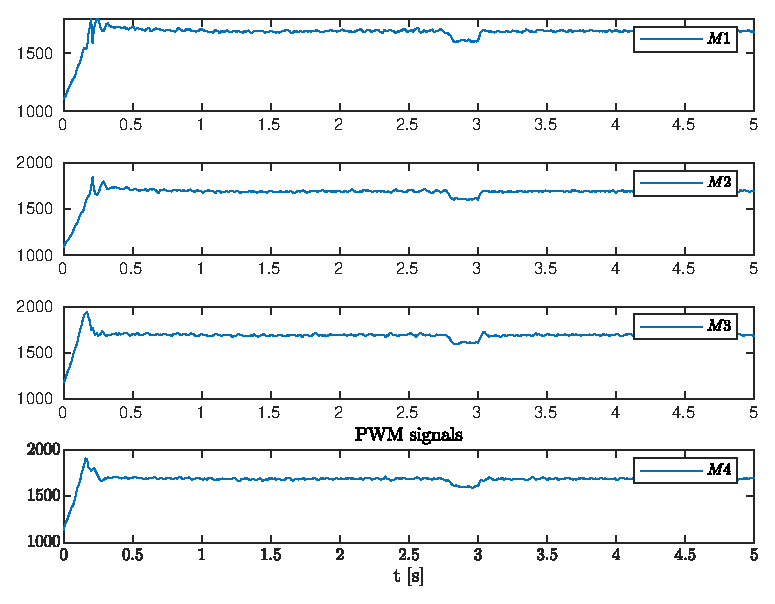
\includegraphics[width=0.45\textwidth]{Simulazioni/Figure/PID/STEP/PWM}
	\caption{Segnali PWM del controllore PID al segnale STEP}
	\label{fig:STEPerrPWMPID}
\end{figure}

Analizzando i dati di questa simulazione si osserva come il controllore PID risponda correttamente al comando di decollo. L'errore iniziale risulta essere maggiore nella prima fase a causa dell'errore misurato inizialmente sulla quota. Nel proseguire della manovra il sistema riesce correttamente a minimizzare corettamente l'errore di posizione, Figura (\ref{fig:STEPerrposzPID}). L'inseguimento del rateo di salita risulta essere imprecisa nella fase iniziale, presentando un overshoot e un successivo assestamento lento è impreciso. Nella fase di livellamento però sia l'overshoot che l'errore stazionario si riduce, Figura (\ref{fig:STEPerrposzPID}). Il segnale PWM in uscita del controllore risulta essere abbastanza regolare, senza presentare oscillazioni eccessive, rimanendo in un range nominale e non presentando saturazione, Figura(\ref{fig:STEPerrPWMPID}).

La seconda simulazione, prevede di attuare il profilo di missione descritto nella Tabella (\ref{tab:SQUARE}). Il segnale di riferimento generato in termine di velocità, di colore rosso nelle Figure (\ref{fig:SQUAREerrposxPID}) e (\ref{fig:SQUAREerrposyPID}), come nel caso precedente è di forma trapezoidale raccordato. Al raggiungimento del waypoint viene annullata la velocità, mentre nella traslazione a regime la velocità comandata è di circa  0.6 m/s. Nelle Figure (\ref{fig:SQUAREerrposxPID}) e (\ref{fig:SQUAREerrposyPID}) vengono mostrate in colore rosso i segnali generati necessari a percorrere la traiettoria simulata. Questi hanno sostanzialmente una forma triangolare raccordati nei punti di variazione di velocità con alcuni tratti costanti.

\begin{figure}
	\centering
	\begin{subfigure}{0.45\textwidth}
		\centering
		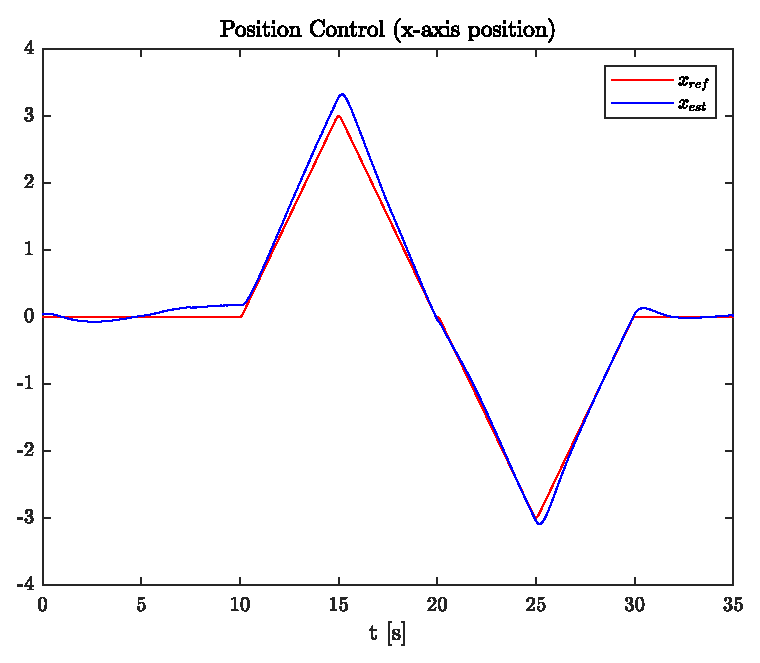
\includegraphics[width=1\textwidth]{Simulazioni/Figure/PID/SQUARE/PositionControlXPos}
		\caption{Controllo posizione lungo x}
		\label{fig:SQUAREerrposxPID}
	\end{subfigure}
	\hfill
	\begin{subfigure}{0.45\textwidth}
		\centering
		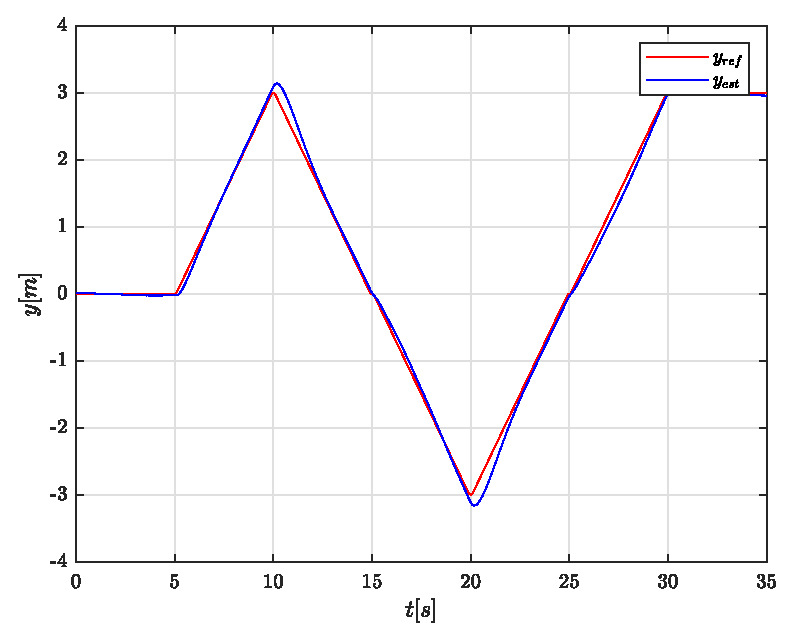
\includegraphics[width=1\textwidth]{Simulazioni/Figure/PID/SQUARE/PositionControlYPos}
		\caption{Controllo posizione lungo y}
		\label{fig:SQUAREerrposyPID}
	\end{subfigure}
	\caption{Risposta in posizione con controllore PID al comando SQUARE}
\end{figure}
\begin{figure}
	\centering
	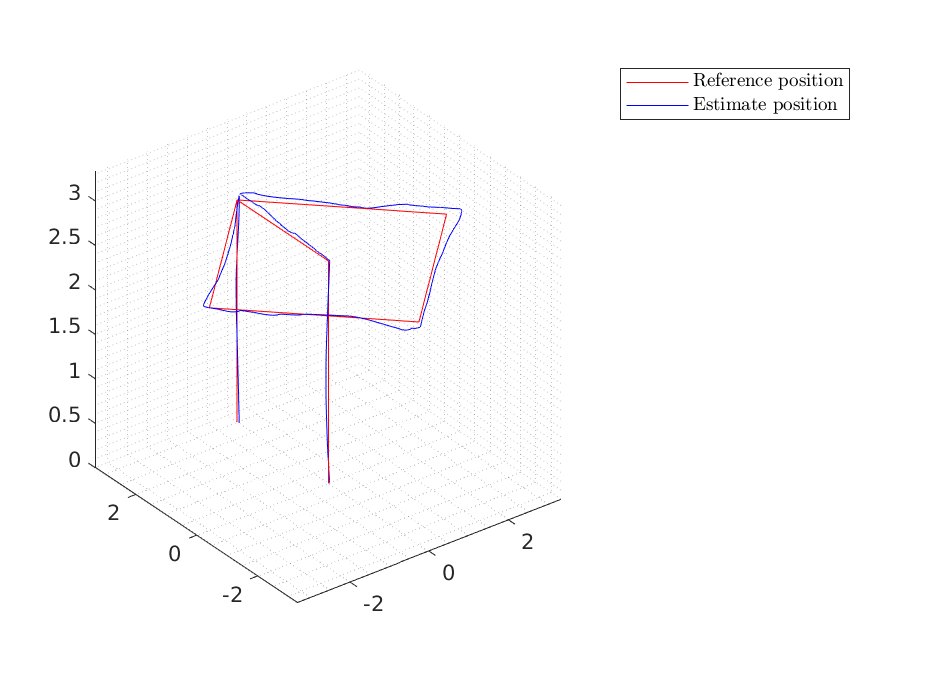
\includegraphics[width=0.65\textwidth]{Simulazioni/Figure/PID/SQUARE/Trajectory}
	\caption{Traiettoria percorsa con controllore PID al comando SQUARE}
	\label{fig:SQUAREtraPID}
\end{figure}

\begin{figure}
	\centering
	\begin{subfigure}{0.45\textwidth}
		\centering
		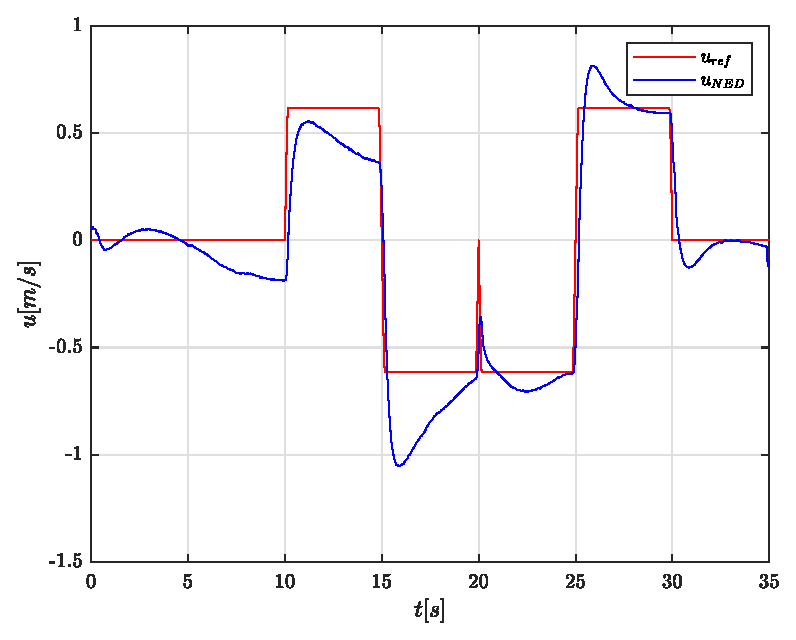
\includegraphics[width=1\textwidth]{Simulazioni/Figure/PID/SQUARE/PositionControlXVel}
		\caption{Controllo velocità lungo x}
		\label{fig:SQUAREerrvelxPID}
	\end{subfigure}
	\hfill
	\begin{subfigure}{0.45\textwidth}
		\centering
		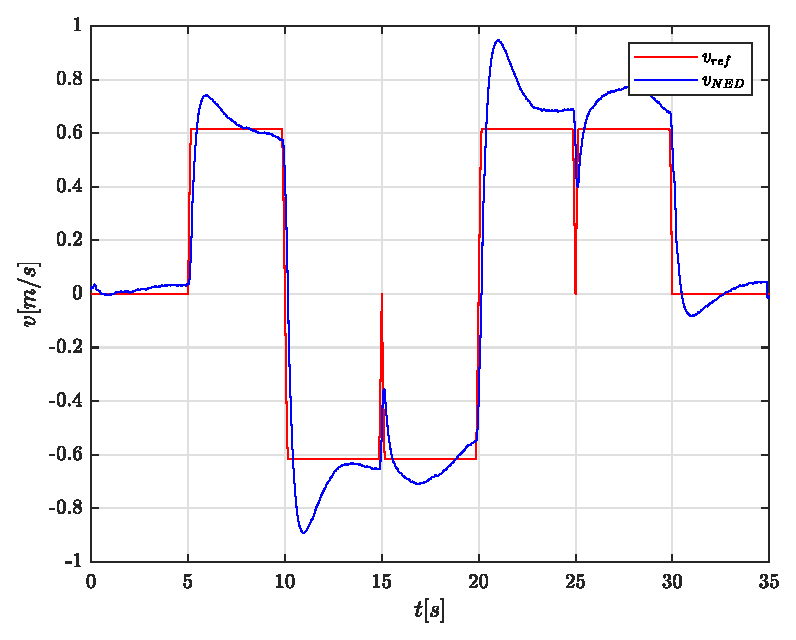
\includegraphics[width=1\textwidth]{Simulazioni/Figure/PID/SQUARE/PositionControlYVel}
		\caption{Controllo velocità lungo y}
		\label{fig:SQUAREerrvelyPID}
	\end{subfigure}
	\caption{Risposta in velocità con controllore PID al comando SQUARE}
\end{figure}

\begin{figure}
	\centering
	\begin{subfigure}{0.45\textwidth}
		\centering
		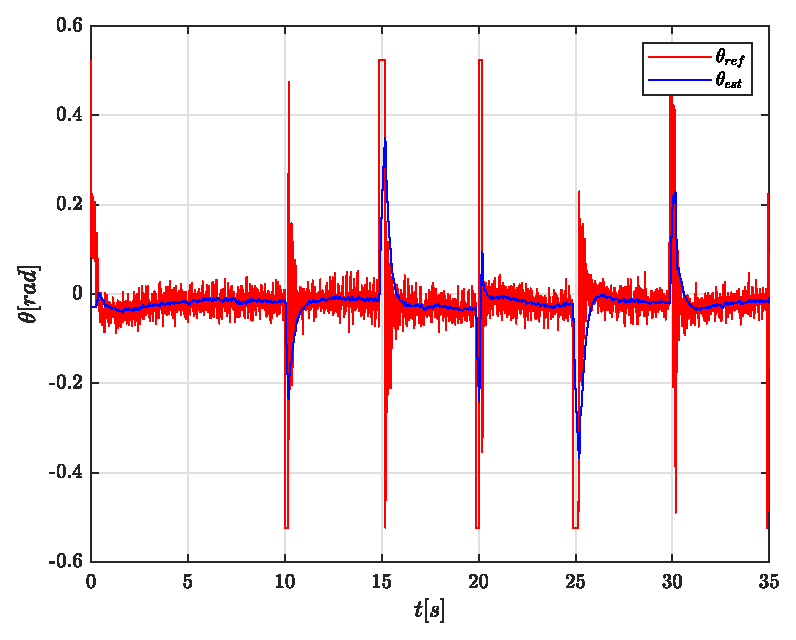
\includegraphics[width=1\textwidth]{Simulazioni/Figure/PID/SQUARE/AttitudeControlPitch}
		\caption{Controllo beccheggio}
		\label{fig:SQUAREerrbecPID}
	\end{subfigure}
	\hfill
	\begin{subfigure}{0.45\textwidth}
		\centering
		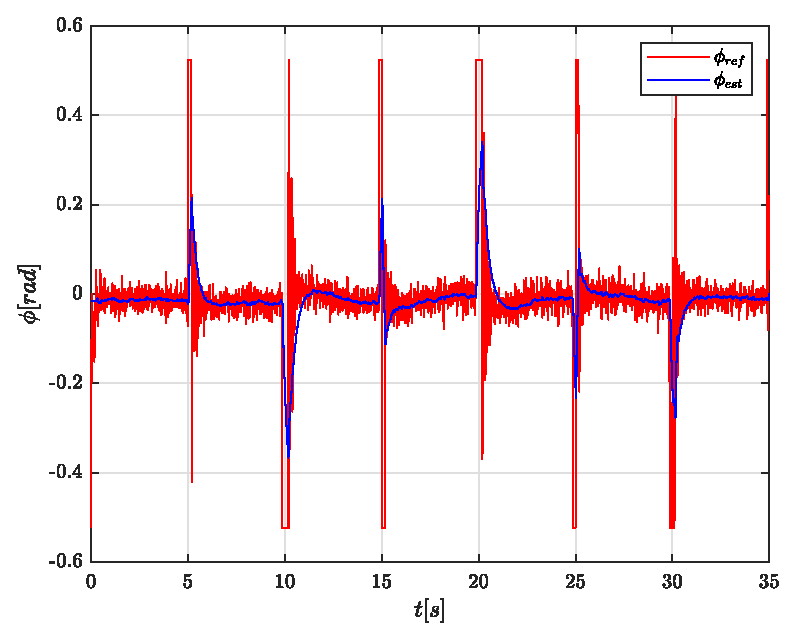
\includegraphics[width=1\textwidth]{Simulazioni/Figure/PID/SQUARE/AttitudeControlRoll}
		\caption{Controllo rollio}
		\label{fig:SQUAREerrrolPID}
	\end{subfigure}
	\hfill
	\begin{subfigure}{0.45\textwidth}
		\centering
		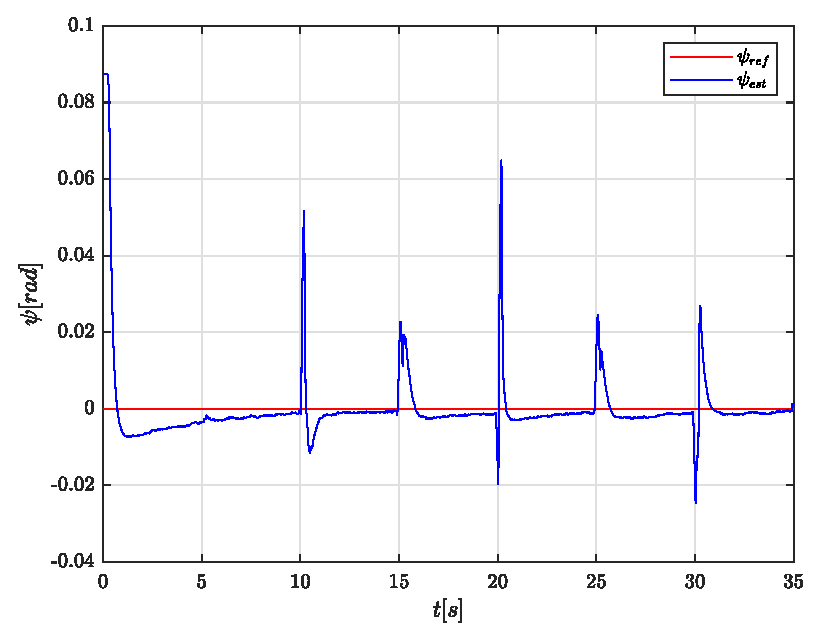
\includegraphics[width=1\textwidth]{Simulazioni/Figure/PID/SQUARE/AttitudeControlYaw}
		\caption{Controllo imbardata}
		\label{fig:SQUAREerryawPID}
	\end{subfigure}
	\caption{Risposta dell' assetto con controllore PID al comando SQUARE}
\end{figure}


\begin{figure}
	\centering
	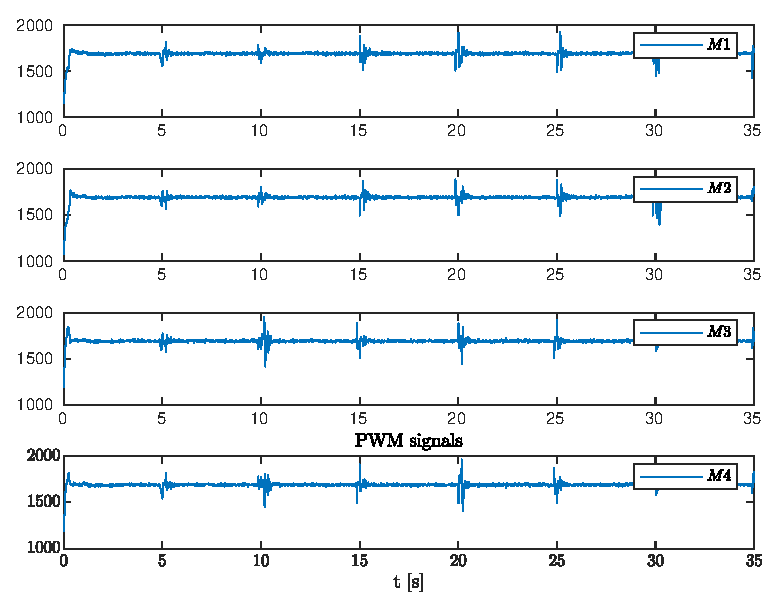
\includegraphics[width=0.45\textwidth]{Simulazioni/Figure/PID/SQUARE/PWM}
	\caption{Segnali PWM del controllore PID al segnale SQUARE}
	\label{fig:SQUAREPWMPID}
\end{figure}

Analizzando questa simulazione viene mostrata la capacità di muoversi nello spazio rispetto alle coordinate $x$ e $y$. L'errore di posizione osservato risulta essere relativamente piccolo. Gli incrementi di questo risultano essere maggiori nella fase di decollo iniziale e nell'attuazione dei cambi di velocità, Figure (\ref{fig:SQUAREerrposxPID}) e (\ref{fig:SQUAREerrposyPID}). L'inseguimento da parte del controllore PID nei confronti della velocità presenta alcuni picchi di overshoot quando questa subisce repentine variazioni, mostrando però l'assestamento successivo verso la riduzione asintotica della differenza. La risposta in velocità risulta essere molto rapida, Figure (\ref{fig:SQUAREerrvelxPID}) e (\ref{fig:SQUAREerrvelyPID}). Osservando i segnali di riferimento generati dal Position Control per l'Attitude Control,nelle Figure (\ref{fig:SQUAREerrbecPID}) e (\ref{fig:SQUAREerrrolPID}), si nota la presenza di intervalli in cui il controllore di posizione è in saturazione. Il segnale di riferimento generato dal Position Control presenta una componente di rumore. Il velivolo riesce comunque a seguire mediamente questo segnale, portandosi in condizione di assetto corretto per seguire la velocità di traslazione. Per quanto riguarda l'angolo di imbardata, con riferimento costante, presenta a causa degli effetti di accoppiamento tra le rotazioni lungo gli assi $x$ e $y$, degli scostamenti. Il sistema risponde molto bene per ridurre questo tipo di errore, come è osservabile nella Figura (\ref{fig:SQUAREerryawPID}). Anche in questa simulazione il segnale PWM generato è molto pulito e non presenta oscillazioni di ampiezza rilevante rispetto al valore medio, Figura (\ref{fig:SQUAREPWMPID}). Osservando la Figura (\ref{fig:SQUAREtraPID}), si osserva come il controllore sia in grado di percorrere la traiettoria prestabilita in modo efficacie, con alcune fasi di scostamento nelle variazione della direzione. La fase di atterraggio non presenta particolari criticità.

Nella successiva simulazione viene mostrata la risposta riguardante il segnale di riferimento generato per la missione BUTTERFLY, missione riassunta nella Tabella(\ref{tab:BUTTERFLY}) e descritta in precedenza. Il segnale di riferimento relativo alla velocità , Figure (\ref{fig:BUTTERFLYerrvelxPID}) e (\ref{fig:BUTTERFLYerrvelyPID}), è analogo alle due simulazioni precedenti con velocità a regime di circa 1.25 m/s. Il profilo di posizione di riferimento di posizione lungo l'asse $x$ ha una forma trapezoidale con raccordi in prossimità delle variazioni di velocità e alcuni tratti costanti, Figura (\ref{fig:BUTTERFLYerrposxPID}). Il profilo di riferimento riguardante la posizione $y$, invece è analogo alla simulazione precedente, Figura (\ref{fig:BUTTERFLYerrposyPID}).

\begin{figure}
	\centering
	\begin{subfigure}{0.45\textwidth}
		\centering
		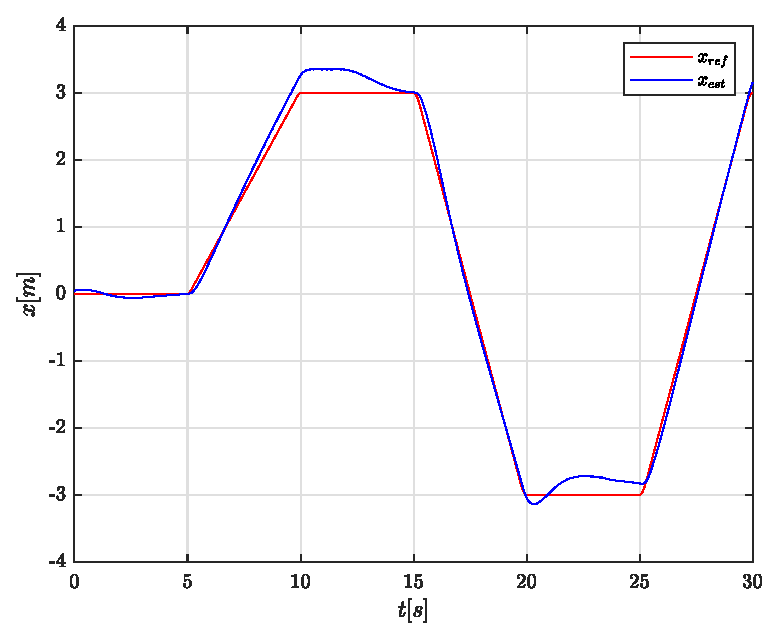
\includegraphics[width=1\textwidth]{Simulazioni/Figure/PID/BUTTERFLY/PositionControlXPos}
		\caption{Controllo posizione lungo x}
		\label{fig:BUTTERFLYerrposxPID}
	\end{subfigure}
	\hfill
	\begin{subfigure}{0.45\textwidth}
		\centering
		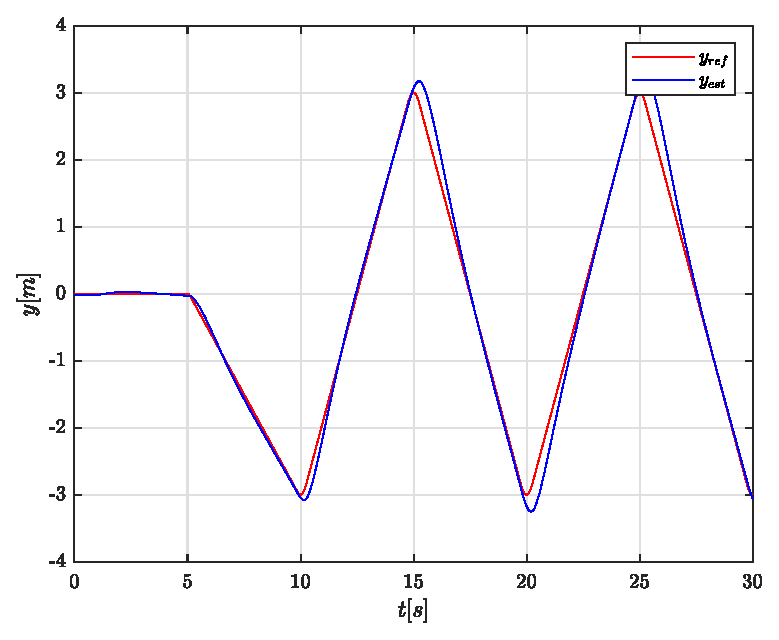
\includegraphics[width=1\textwidth]{Simulazioni/Figure/PID/BUTTERFLY/PositionControlYPos}
		\caption{Controllo posizione lungo y}
		\label{fig:BUTTERFLYerrposyPID}
	\end{subfigure}
	\caption{Risposta in posizione con controllore PID al comando BUTTERFLY}
\end{figure}

\begin{figure}
	\centering
	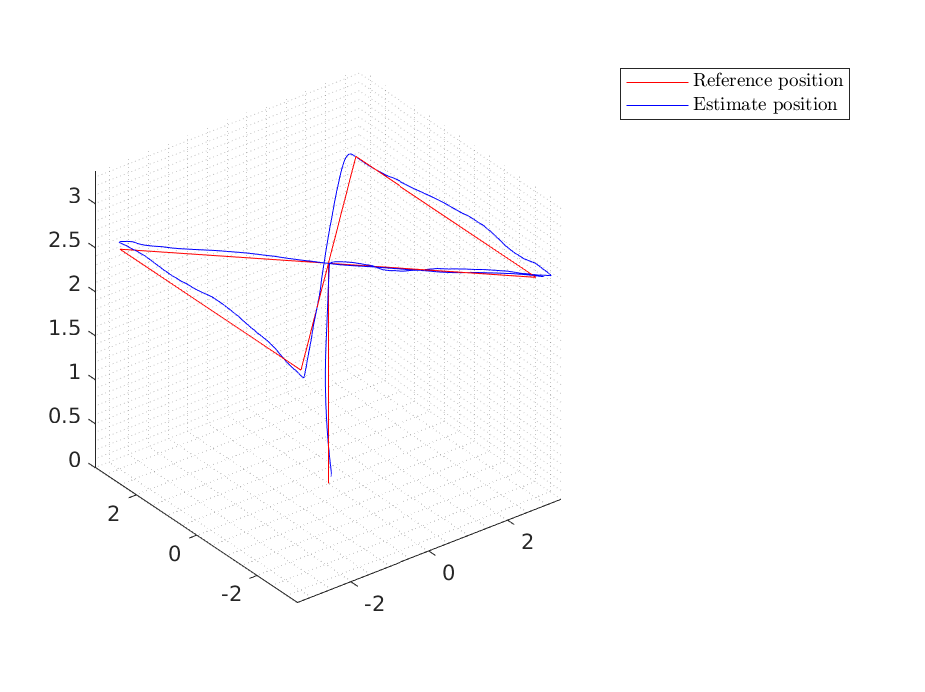
\includegraphics[width=0.65\textwidth]{Simulazioni/Figure/PID/BUTTERFLY/Trajectory}
	\caption{Traiettoria percorsa con controllore PID al comando BUTTERFLY}
	\label{fig:BUTTERFLYtraPID}
\end{figure}

\begin{figure}
	\centering
	\begin{subfigure}{0.45\textwidth}
		\centering
		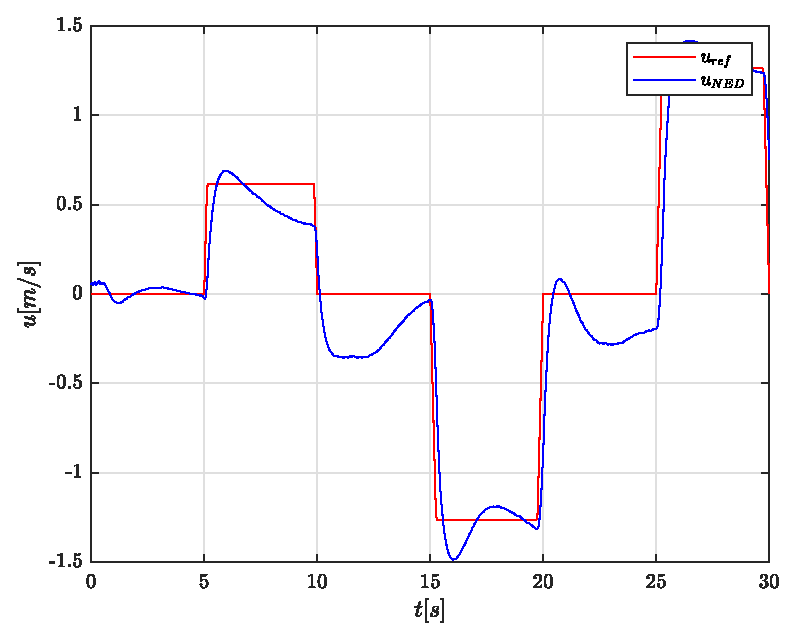
\includegraphics[width=0.65\textwidth]{Simulazioni/Figure/PID/BUTTERFLY/PositionControlXVel}
		\caption{Controllo velocità lungo x}
		\label{fig:BUTTERFLYerrvelxPID}
	\end{subfigure}
	\hfill
	\begin{subfigure}{0.45\textwidth}
		\centering
		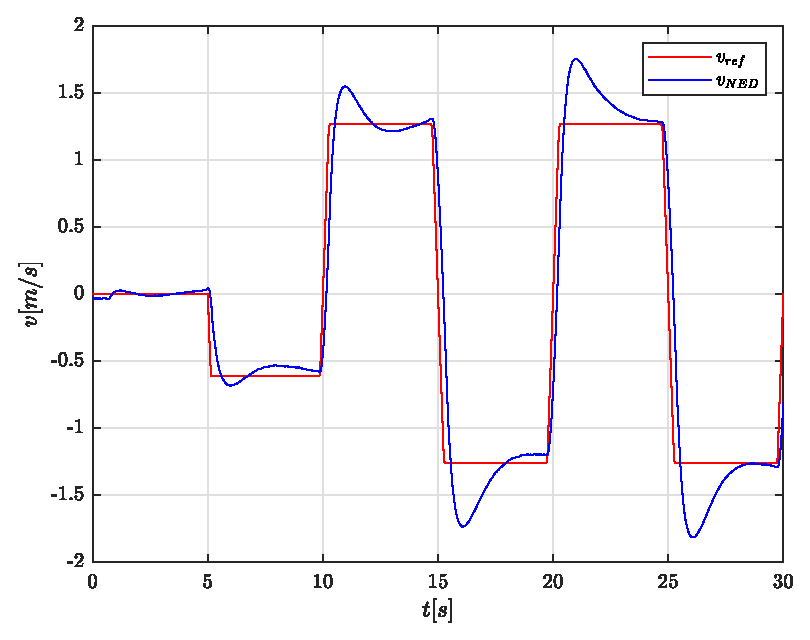
\includegraphics[width=1\textwidth]{Simulazioni/Figure/PID/BUTTERFLY/PositionControlYVel}
		\caption{Controllo velocità lungo y}
		\label{fig:BUTTERFLYerrvelyPID}
	\end{subfigure}
		\caption{Risposta in velocità con controllore PID al comando BUTTERFLY}
\end{figure}

\begin{figure}
	\centering
	\begin{subfigure}{0.45\textwidth}
		\centering
		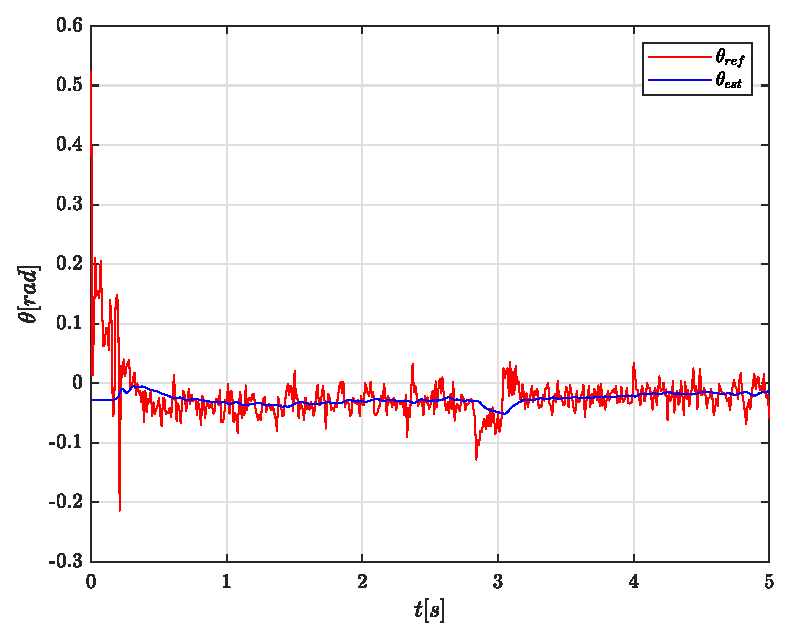
\includegraphics[width=1\textwidth]{Simulazioni/Figure/PID/BUTTERFLY/AttitudeControlPitch}
		\caption{Controllo beccheggio}
		\label{fig:BUTTERFLYerrbecPID}
	\end{subfigure}
	\hfill
	\begin{subfigure}{0.45\textwidth}
		\centering
		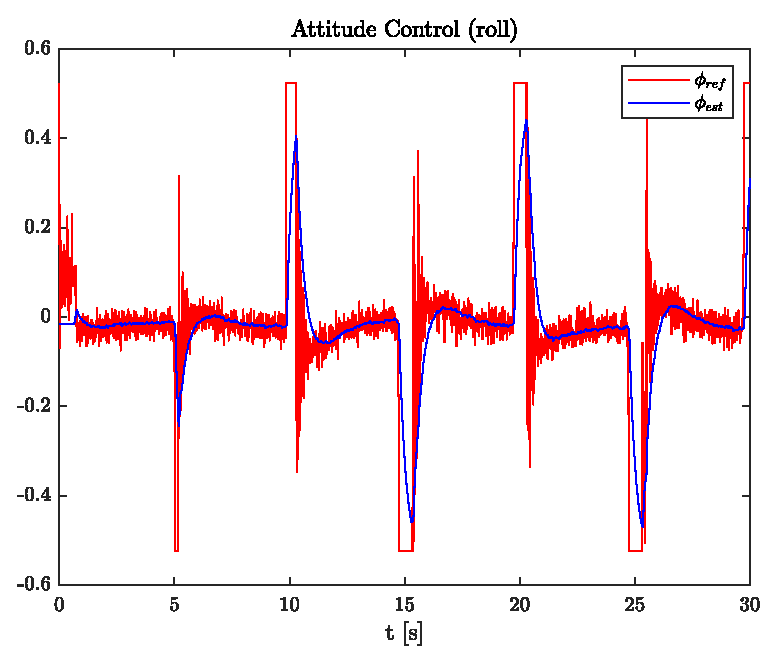
\includegraphics[width=1\textwidth]{Simulazioni/Figure/PID/BUTTERFLY/AttitudeControlRoll}
		\caption{Controllo rollio}
		\label{fig:BUTTERFLYerrrolPID}
	\end{subfigure}
	\hfill
	\begin{subfigure}{0.45\textwidth}
		\centering
		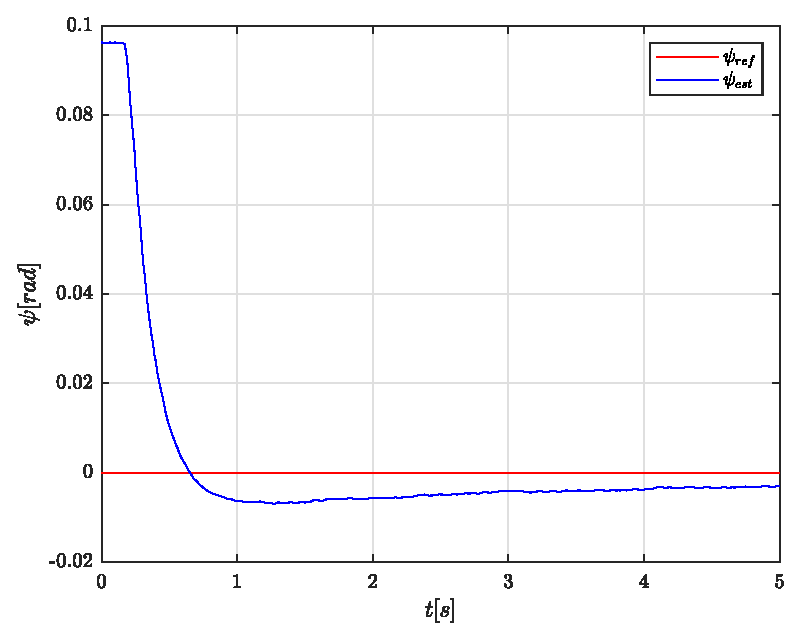
\includegraphics[width=1\textwidth]{Simulazioni/Figure/PID/BUTTERFLY/AttitudeControlYaw}
		\caption{Controllo imbardata}
		\label{fig:BUTTERFLYerryawPID}
	\end{subfigure}
	\caption{Risposta dell' assetto con controllore PID al comando BUTTERFLY}
\end{figure}


\begin{figure}
	\centering
	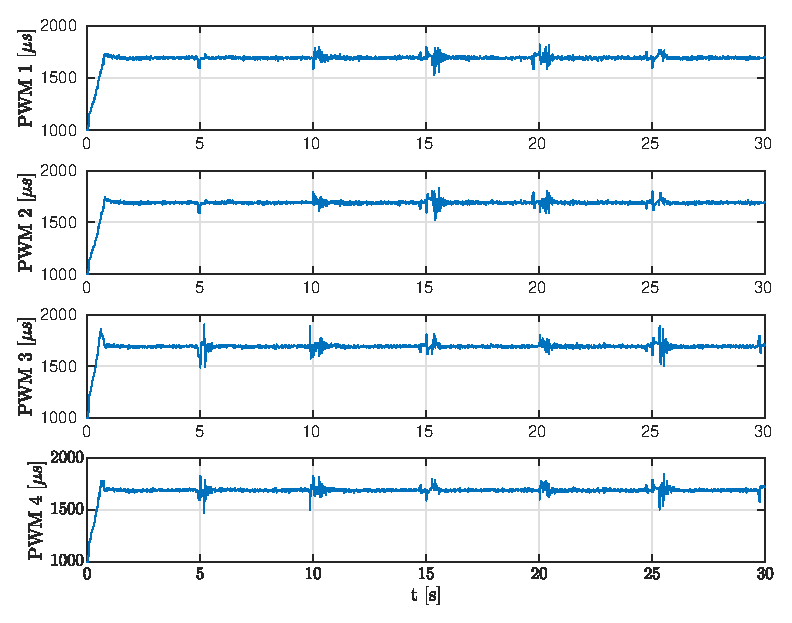
\includegraphics[width=0.45\textwidth]{Simulazioni/Figure/PID/BUTTERFLY/PWM}
	\caption{Segnali PWM del controllore PID al segnale BUTTERFLY}
	\label{fig:BUTTERFLYPWMPID}
\end{figure}

Nella simulazione analizzata, viene eseguito un percorso più lungo rispetto alla precedente in termine di spazio percorso, inoltre il cambiamento di direzione comandato al raggiungimento del waypoint è maggiore. La risposta è molto simile alla precedente. Anche in questa simulazione l'errore di posizione osservato risulta essere piccolo. Gli incrementi risultano maggiori nella fase di decollo iniziale e nell'attuazione dei cambi di velocità, Figure (\ref{fig:BUTTERFLYerrposxPID}) e (\ref{fig:BUTTERFLYerrposyPID}). Sono presenti i picchi di overshoot nella risposta in velocità, con una fase successiva di assestamento. La risposta in velocità è rapida, Figure (\ref{fig:BUTTERFLYerrvelxPID}) e (\ref{fig:BUTTERFLYerrvelyPID}). Nelle Figure (\ref{fig:BUTTERFLYerrbecPID}) e (\ref{fig:BUTTERFLYerrrolPID}), si nota la presenza di intervalli in cui il controllore di posizione è in saturazione e la presenza di un oscillazione rispetto ad un valore medio. Il segnale PWM generato è molto pulito e non presenta oscillazioni di ampiezza rilevante rispetto al valore medio, Figura (\ref{fig:BUTTERFLYPWMPID}). Come osservabile in Figura (\ref{fig:BUTTERFLYtraPID}), il controllore è in grado di percorrere efficacemente la traiettoria prestabilita con alcuni scostamenti in presenza di cambiamenti repentini di direzione.

La seconda simulazione, prevede di attuare il profilo di missione descritto nella Tabella (\ref{tab:SQUARE}). Questo profilo è il più complesso tra quelli presentati. Il profili di velocità hanno una forma trapezoidale raccordata in prossimità delle variazioni di velocità, di valore circa 0.6 m/s a regime, Figura (\ref{fig:SNAKEerrvelxPID}) e (\ref{fig:SNAKEerrvelyPID}). La relativa forma del segnale di riferimento della posizione lungo l'asse $x$ è simile alle simulazioni precedenti, Figura (\ref{fig:SNAKEerrposxPID}), mentre lungo l'asse $y$ il profilo presenta, sempre con raccordi in prossimità della variazione di velocità, sia forma triangolare che trapezoidale con una porzione formata da tratti lineari e costanti, Figura (\ref{fig:SNAKEerrposyPID}).

\begin{figure}
	\centering
	\begin{subfigure}{0.45\textwidth}
		\centering
		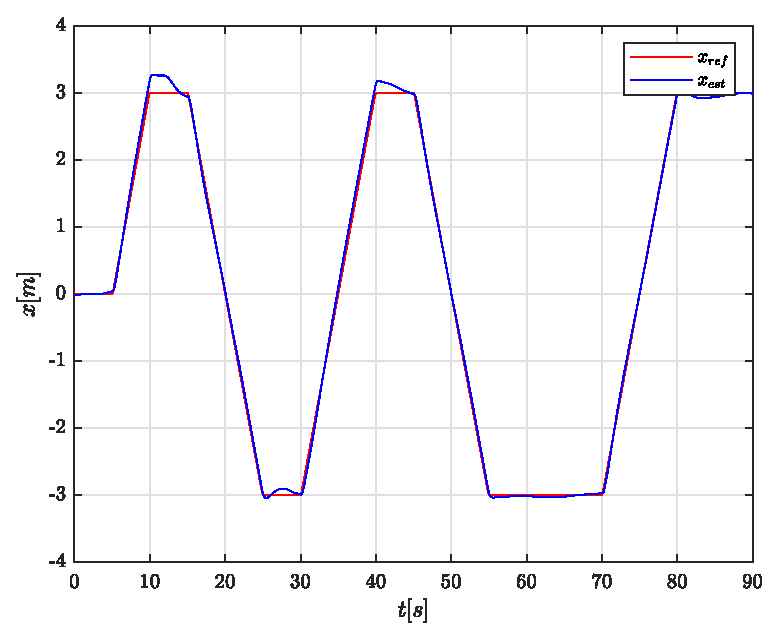
\includegraphics[width=1\textwidth]{Simulazioni/Figure/PID/SNAKE/PositionControlXPos}
		\caption{Controllo posizione lungo x}
		\label{fig:SNAKEerrposxPID}
	\end{subfigure}
	\hfill
	\begin{subfigure}{0.45\textwidth}
		\centering
		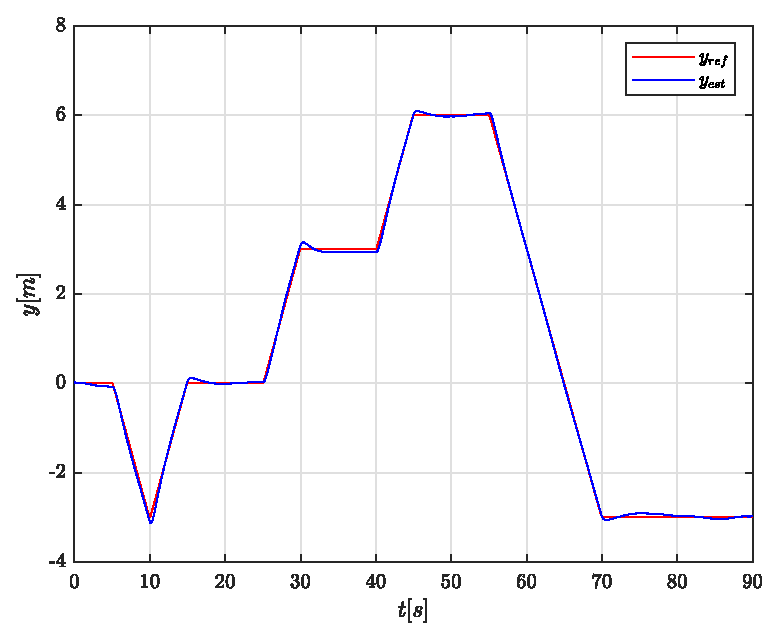
\includegraphics[width=1\textwidth]{Simulazioni/Figure/PID/SNAKE/PositionControlYPos}
		\caption{Controllo posizione lungo y}
		\label{fig:SNAKEerrposyPID}
	\end{subfigure}
	\caption{Risposta in posizione con controllore PID al comando SNAKE}
\end{figure}

\begin{figure}
	\centering
	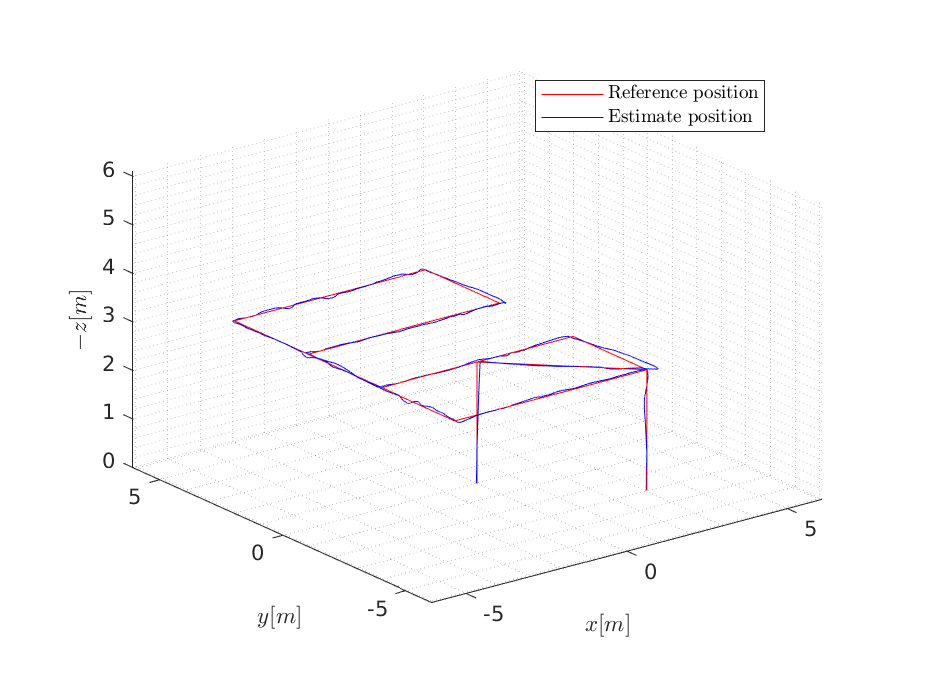
\includegraphics[width=0.65\textwidth]{Simulazioni/Figure/PID/SNAKE/Trajectory}
	\caption{Traiettoria percorsa con controllore PID al segnale SNAKE}
	\label{fig:SNAKEtraPID}
\end{figure}

\begin{figure}
	\centering
	\begin{subfigure}{0.45\textwidth}
		\centering
		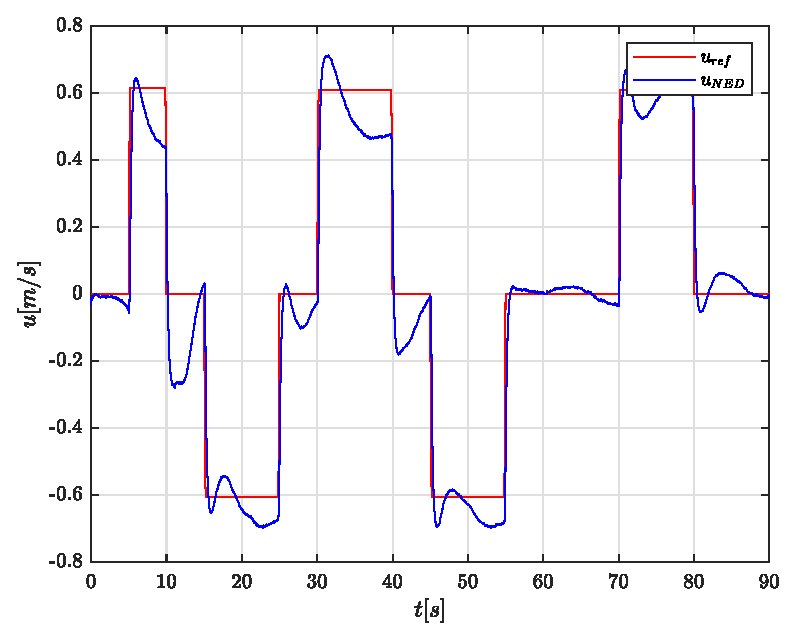
\includegraphics[width=1\textwidth]{Simulazioni/Figure/PID/SNAKE/PositionControlXVel}
		\caption{Controllo velocità lungo x}
		\label{fig:SNAKEerrvelxPID}
	\end{subfigure}
	\hfill
	\begin{subfigure}{0.45\textwidth}
		\centering
		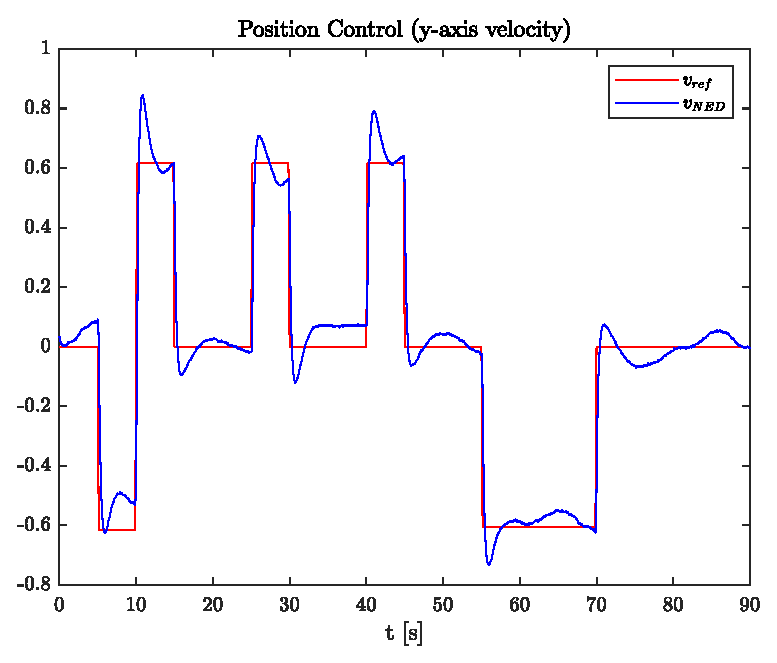
\includegraphics[width=1\textwidth]{Simulazioni/Figure/PID/SNAKE/PositionControlYVel}
		\caption{Controllo velocità lungo y}
		\label{fig:SNAKEerrvelyPID}
	\end{subfigure}
	\caption{Risposta in velocità con controllore PID al comando SNAKE}
\end{figure}

\begin{figure}
	\centering
	\begin{subfigure}{0.45\textwidth}
		\centering
		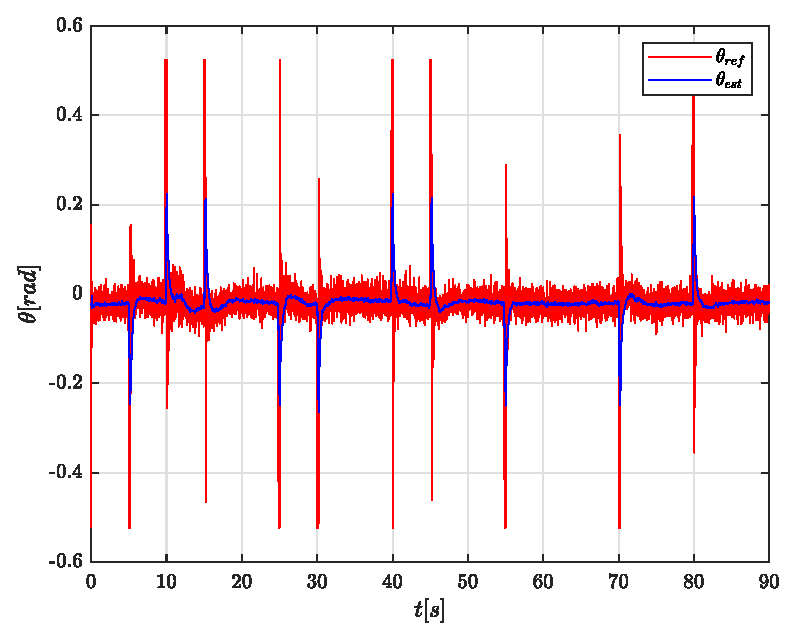
\includegraphics[width=1\textwidth]{Simulazioni/Figure/PID/SNAKE/AttitudeControlPitch}
		\caption{Controllo beccheggio}
		\label{fig:SNAKEerrbecPID}
	\end{subfigure}
	\hfill
	\begin{subfigure}{0.45\textwidth}
		\centering
		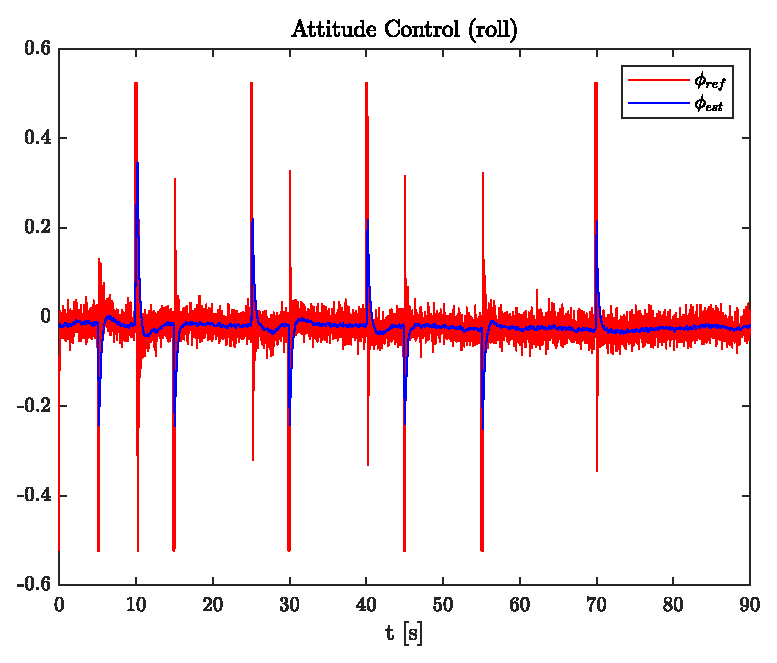
\includegraphics[width=1\textwidth]{Simulazioni/Figure/PID/SNAKE/AttitudeControlRoll}
		\caption{Controllo rollio}
		\label{fig:SNAKEerrrolPID}
	\end{subfigure}
	\hfill
	\begin{subfigure}{0.45\textwidth}
		\centering
		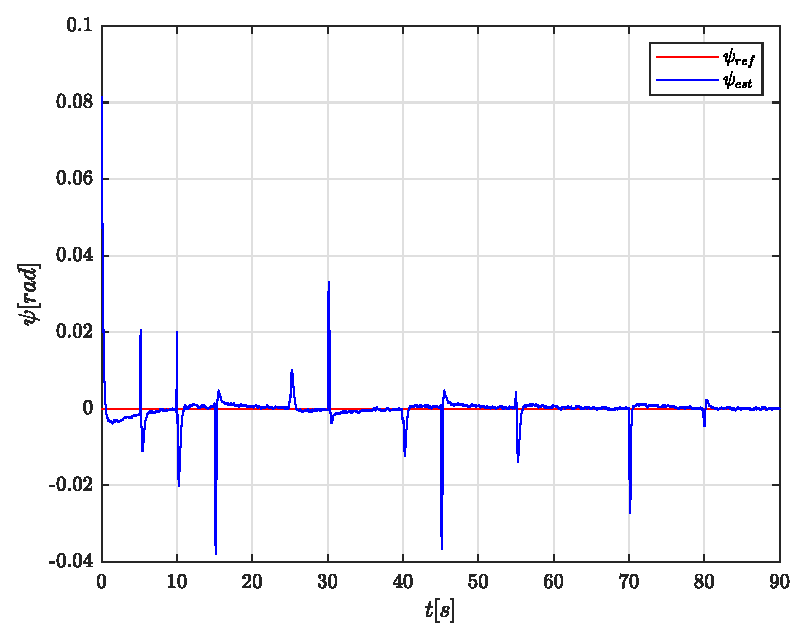
\includegraphics[width=1\textwidth]{Simulazioni/Figure/PID/SNAKE/AttitudeControlYaw}
		\caption{Controllo imbardata}
		\label{fig:SNAKEerryawPID}
	\end{subfigure}
	\caption{Risposta dell' assetto con controllore PID al comando SNAKE}
\end{figure}

\begin{figure}
	\centering
	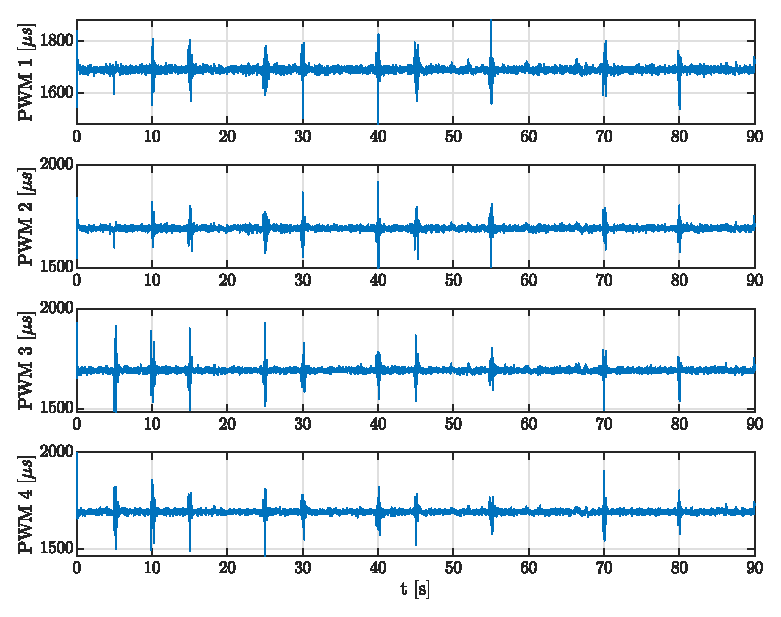
\includegraphics[width=0.45\textwidth]{Simulazioni/Figure/PID/SNAKE/PWM}
	\caption{Segnali PWM del controllore PID al segnale SNAKE}
	\label{fig:SNAKEPWMPID}
\end{figure}

Infine, in questa simulazione dove viene proposto un percorso più lungo in termine di tempo e spazio percorso, la risposta del sistema riguardante la posizione è precisa, presentando solo piccoli scostamenti nei punti in cui si ha una maggiore variazione di velocità, analogamente alle tre simulazioni mostrate in precedenza, Figure (\ref{fig:SNAKEerrposxPID}) e (\ref{fig:SNAKEerrposyPID}). Anche la risposta in termini di velocità a seguito di oscillazioni tende asintoticamente a rimanere nell'intorno del comando, Figure (\ref{fig:SNAKEerrvelxPID}) e (\ref{fig:SNAKEerrvelyPID}). Anche in questo caso i segnali di riferimento impartiti per gli angoli di beccheggio e rollio presentano delle situazioni di saturazione del cotnrollore di posizione e delle oscillazioni dovute alla presenza dei rumori dei sensori, Figure (\ref{fig:SNAKEerrbecPID}) e (\ref{fig:SNAKEerrrolPID}). La risposta del sistema rispetto all'angolo di imbardata è analogo alle simulazioni precedenti, Figura (\ref{fig:SNAKEerryawPID}). Il segnali PWM generati dal controllore non presentano particolari amplificazioni del rumore o saturazione, (\ref{fig:SNAKEPWMPID}). Osservando la traiettoria percorsa rispetto al riferimento, Figura (\ref{fig:SNAKEtraPID}), si nota l'efficacia del controllore con solo alcuni piccoli scostamenti.

\subsection{SMC}

Vengono qui riportate le simulazioni SIL utilizzando la configurazione denominata SMC nel capitolo \ref{cap:controllore}.

La prima simulazione riguarda il decollo effettuato tramite i segnali definiti dalla pianificazione STEP, come descritto in precedenza. 

\begin{figure}
	\centering
	\begin{subfigure}{0.45\textwidth}
		\centering
		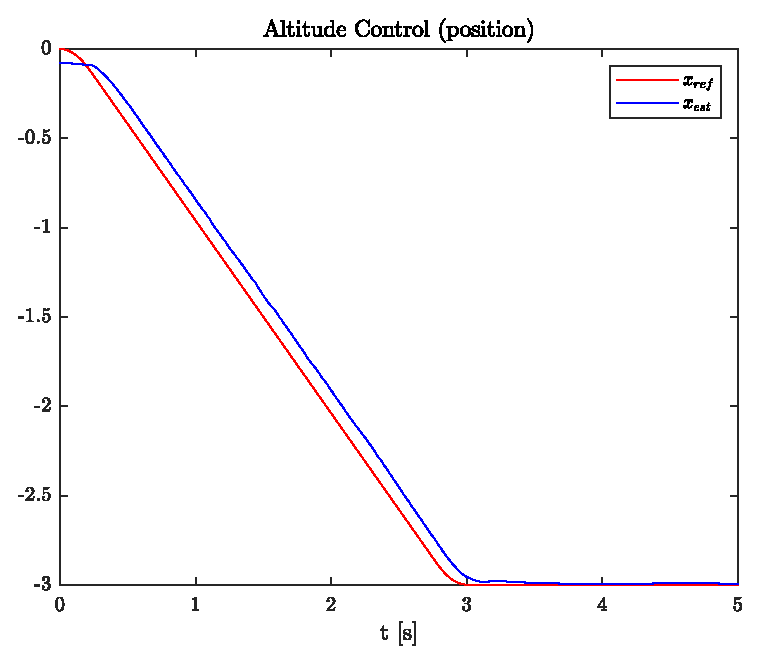
\includegraphics[width=1\textwidth]{Simulazioni/Figure/SMC/STEP/AltitudeControlPos}
		\caption{Controllo posizione}
		\label{fig:STEPerrposzSMC}
	\end{subfigure}
	\hfill
	\begin{subfigure}{0.45\textwidth}
		\centering
		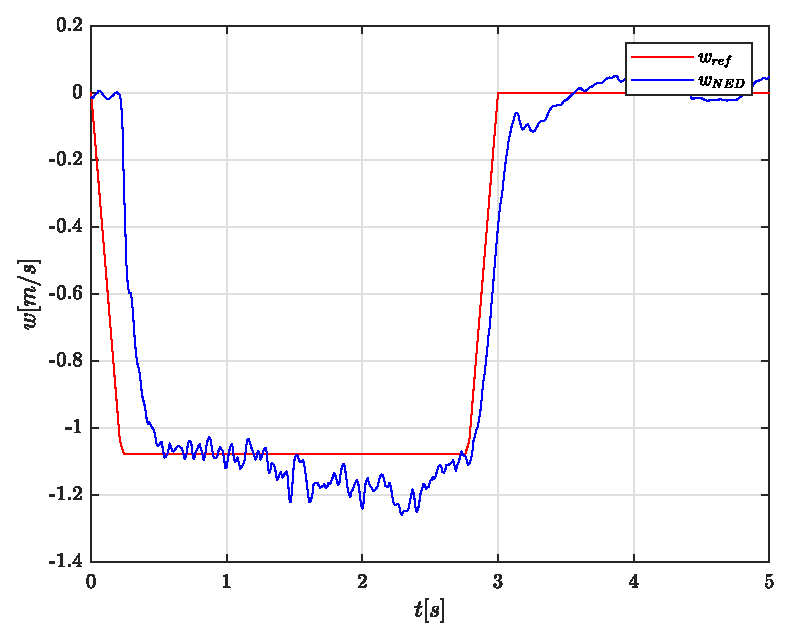
\includegraphics[width=1\textwidth]{Simulazioni/Figure/SMC/STEP/AltitudeControlVel}
		\caption{Controllo velocità}
		\label{fig:STEPerrvelzSMC}
	\end{subfigure}
	\caption{Risposta del controllore SMC di quota al segnale STEP}	
\end{figure}

\begin{figure}
	\centering
	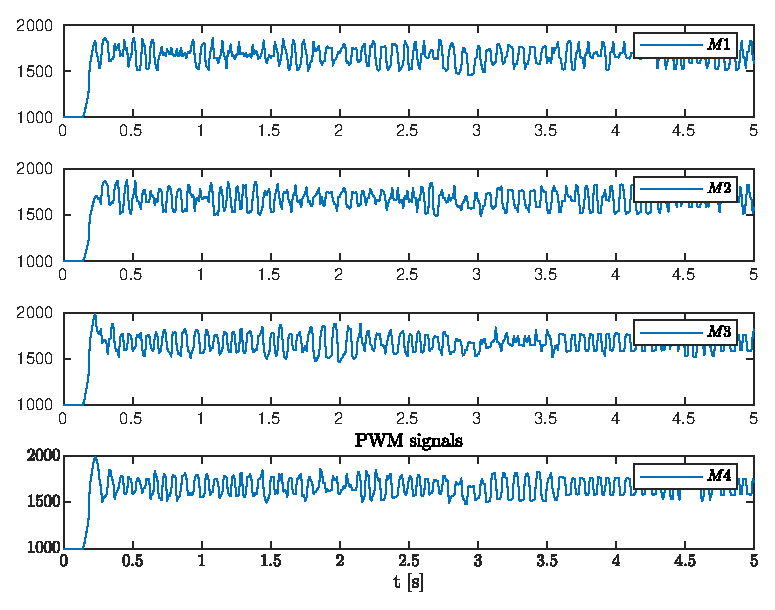
\includegraphics[width=0.45\textwidth]{Simulazioni/Figure/SMC/STEP/PWM}
	\caption{Segnali PWM generati del controllore SMC al segnale STEP}
	\label{fig:STEPPWMSMC}
\end{figure}

La risposta del controllore SMC in merito alla posizione è abbastanza precisa. Sussiste una differenza piccola ma costante lungo tutta la salita, differenza che si annulla rapidamente a livellamento, Figura (\ref{fig:STEPerrposzSMC}). Il profilo di velocità è seguito anch'esso con abbastanza precisione, esiste in questo caso un oscillazione costante nella risposta in velocità rispetto al valore di riferimento della velocità, Figura (\ref{fig:STEPerrvelzSMC}). Il segnale PWM generato da controllore mostra un comportamento discontinuo con ampiezza molto marcata, Figura (\ref{fig:STEPPWMSMC}). 

Viene ora analizzata la traiettoria SQUARE, decritta in precedenza.

\begin{figure}
	\centering
	\begin{subfigure}{0.45\textwidth}
		\centering
		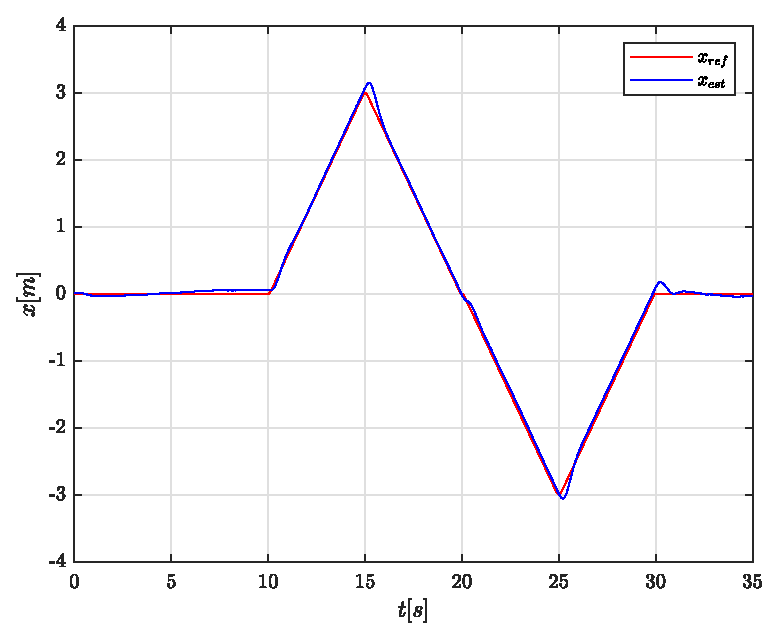
\includegraphics[width=1\textwidth]{Simulazioni/Figure/SMC/SQUARE/PositionControlXPos}
		\caption{Controllo posizione lungo x}
		\label{fig:SQUAREerrposxSMC}
	\end{subfigure}
	\hfill
	\begin{subfigure}{0.45\textwidth}
		\centering
		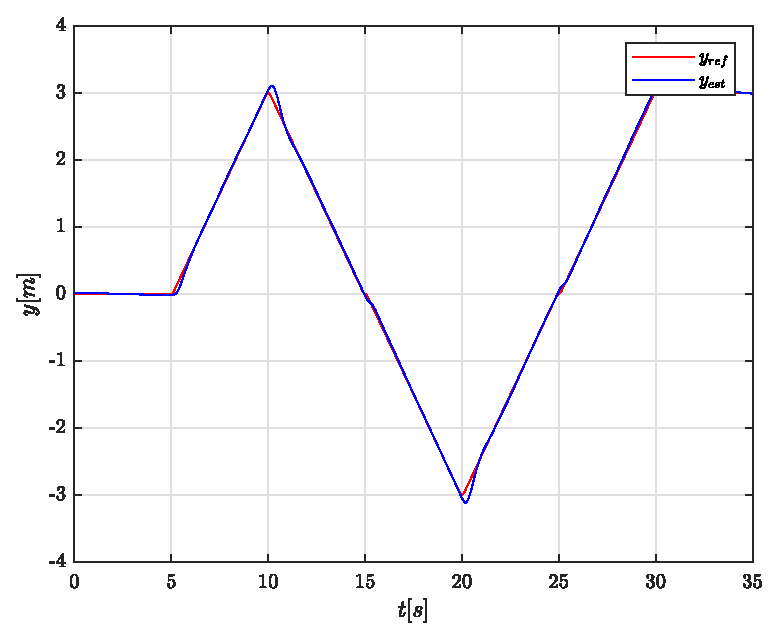
\includegraphics[width=1\textwidth]{Simulazioni/Figure/SMC/SQUARE/PositionControlYPos}
		\caption{Controllo posizione lungo y}
		\label{fig:SQUAREerrposySMC}
	\end{subfigure}
	\caption{Risposta del controllo posizione con controllore SMC al comando SQUARE}
\end{figure}

\begin{figure}
	\centering
	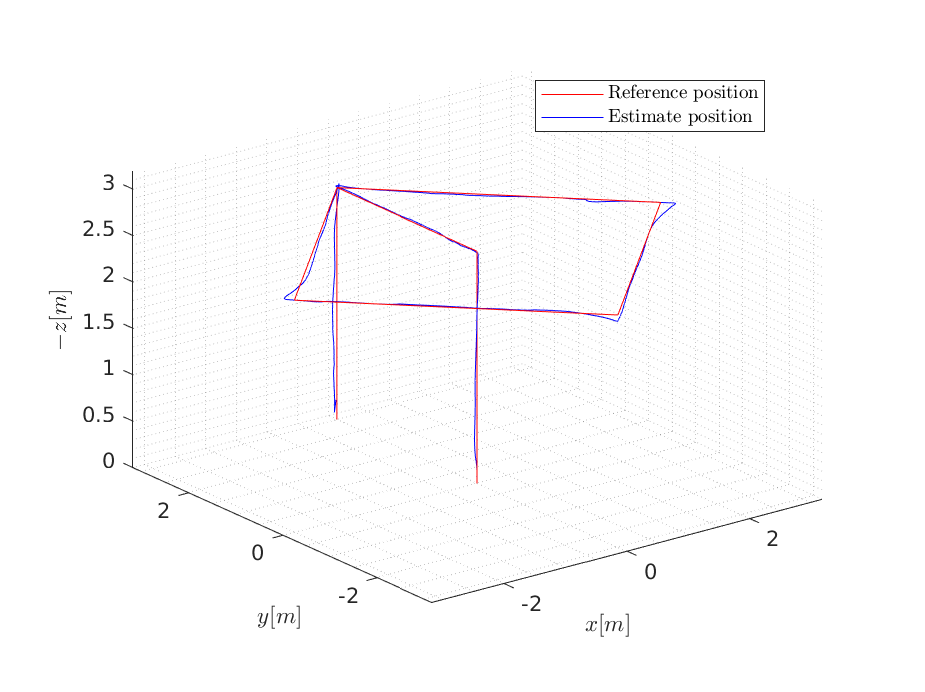
\includegraphics[width=0.65\textwidth]{Simulazioni/Figure/SMC/SQUARE/Trajectory}
	\caption{Traiettoria percorsa con controllore SMC al segnale SQUARE}
	\label{fig:SQUAREtraSMC}
\end{figure}

\begin{figure}
	\centering
	\begin{subfigure}{0.45\textwidth}
		\centering
		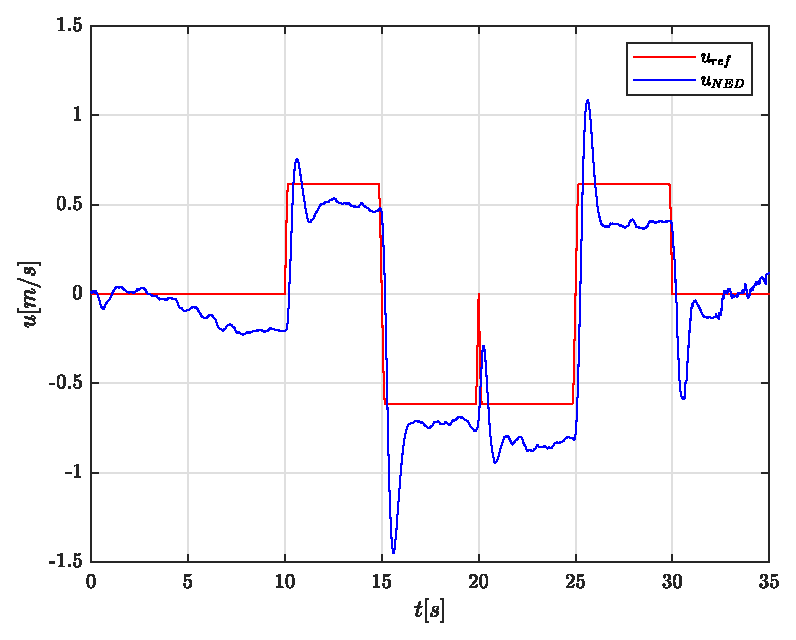
\includegraphics[width=1\textwidth]{Simulazioni/Figure/SMC/SQUARE/PositionControlXVel}
		\caption{Controllo velocità lungo x}
		\label{fig:SQUAREerrvelxSMC}
	\end{subfigure}
	\hfill
	\begin{subfigure}{0.45\textwidth}
		\centering
		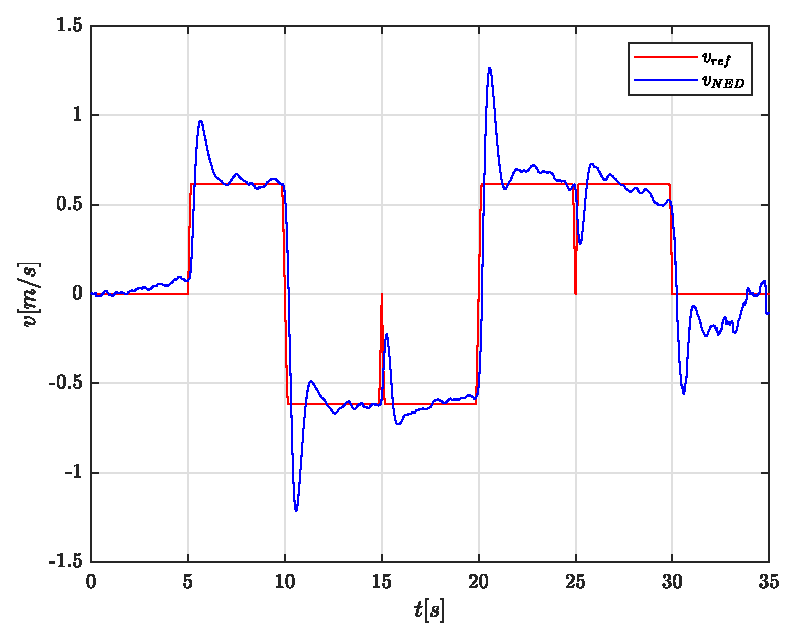
\includegraphics[width=1\textwidth]{Simulazioni/Figure/SMC/SQUARE/PositionControlYVel}
		\caption{Controllo velocità lungo y}
		\label{fig:SQUAREerrvelySMC}
	\end{subfigure}
	\caption{Risposta del controllo velocità con controllore SMC al comando SQUARE}
\end{figure}

\begin{figure}
	\centering
	\begin{subfigure}{0.45\textwidth}
		\centering
		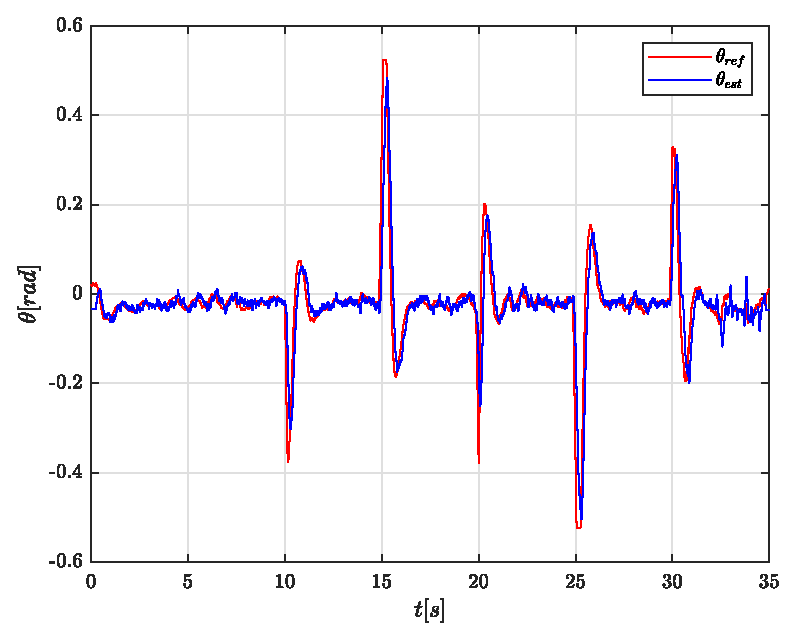
\includegraphics[width=1\textwidth]{Simulazioni/Figure/SMC/SQUARE/AttitudeControlPitch}
		\caption{Controllo beccheggio}
		\label{fig:SQUAREbecSMC}
	\end{subfigure}
	\hfill
	\begin{subfigure}{0.45\textwidth}
		\centering
		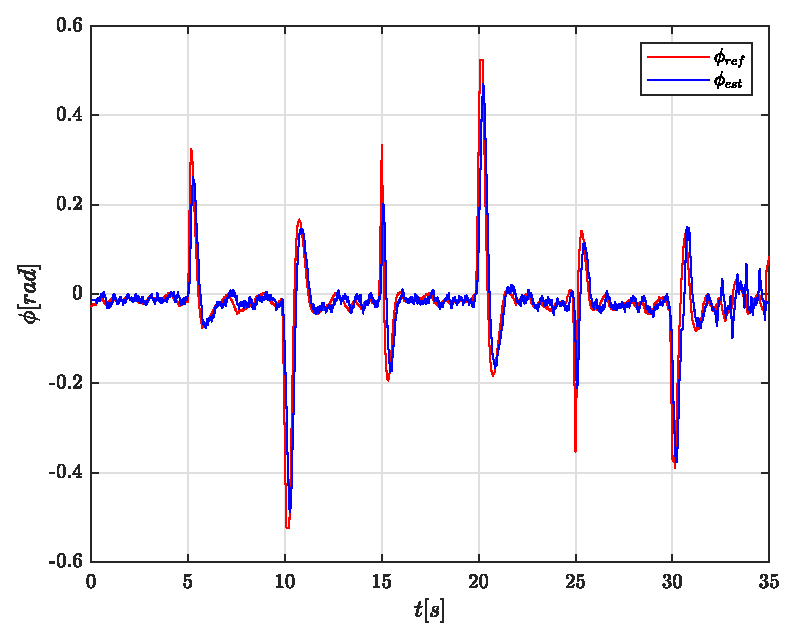
\includegraphics[width=1\textwidth]{Simulazioni/Figure/SMC/SQUARE/AttitudeControlRoll}
		\caption{Controllo rollio}
		\label{fig:SQUARErolSMC}
	\end{subfigure}
	\hfill
	\begin{subfigure}{0.45\textwidth}
		\centering
		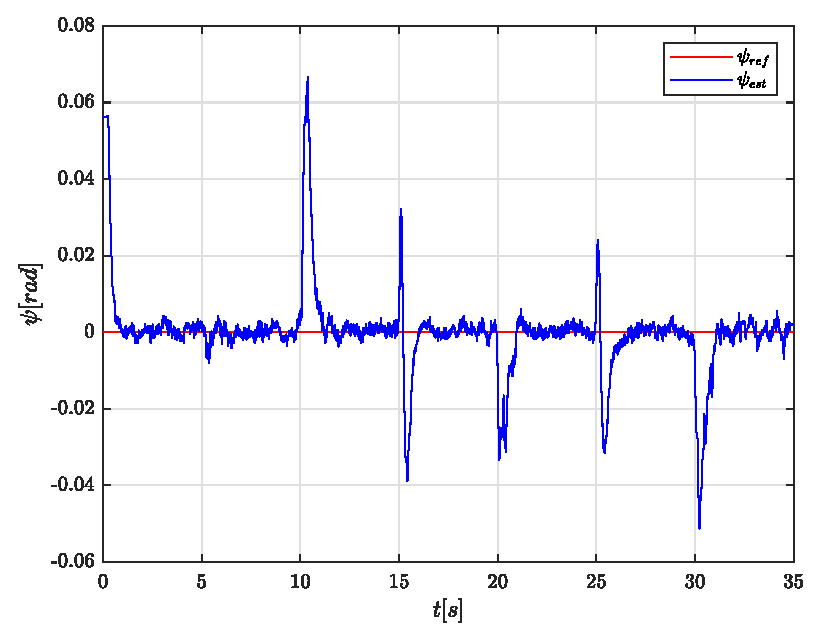
\includegraphics[width=1\textwidth]{Simulazioni/Figure/SMC/SQUARE/AttitudeControlYaw}
		\caption{Controllo imbardata}
		\label{fig:SQUAREyawSMC}
	\end{subfigure}
	\caption{Risposta dell' assetto con controllore SMC al comando SQUARE}
\end{figure}


\begin{figure}
	\centering
	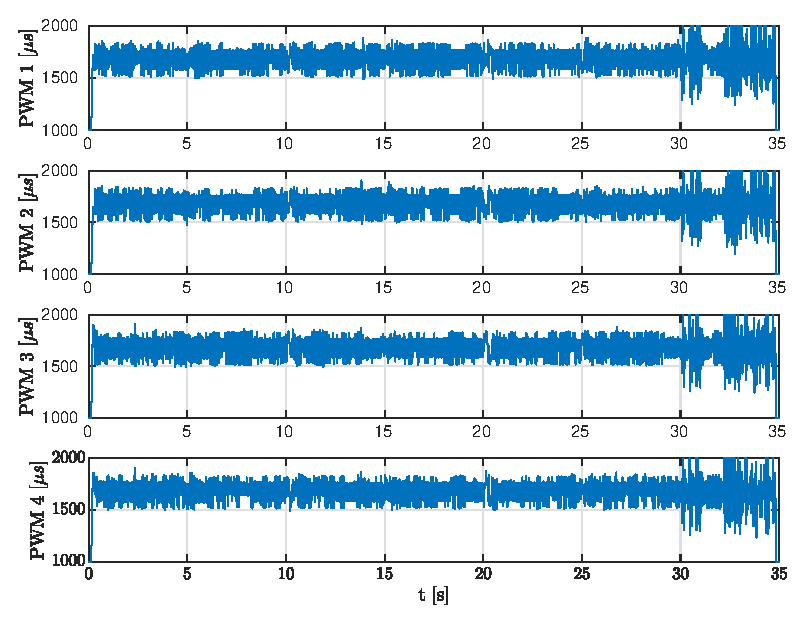
\includegraphics[width=0.45\textwidth]{Simulazioni/Figure/SMC/SQUARE/PWM}
	\caption{Segnali PWM del controllore SMC al segnale SQUARE}
	\label{fig:SQUAREPWMSMC}
\end{figure}


Nella figure (\ref{fig:SQUAREerrposxSMC}) e (\ref{fig:SQUAREerrposySMC}) sono mostrati gli andamenti del drone nel seguire la traiettoria impostaa. In questa simulazione l'errore di posizione è molto ridotto, esiste una differenza osservabile solo nei cambi di direzione, valore molto piccolo. L'inseguimento del profilo di velocità, Figure (\ref{fig:SQUAREerrvelxSMC}) e (\ref{fig:SQUAREerrvelySMC}), avviene con molta precisione e oscillazioni relativamente piccole, presentando alcuni picchi di overshoot nella prossimità dei cambiamenti repentini di velocità, con successivo assestamento. Il segnale di riferimento generato dal comando di posizione non presenta rumore e solo alcune brevi condizioni di saturazione nelle fasi di massima variazione di velocità, Figure (\ref{fig:SQUAREbecSMC}) e (\ref{fig:SQUARErolSMC}). Il sistema di Attitude Control è in grado di seguire questo segnale di riferimento in modo ottimale senza presentare errori eccessivi e oscillazioni. Nella fase terminale del volo, durante la discesa, il comando PWM generato presenta maggiori oscillazioni. Osservando i dati ricavati riguardante il segnale PWM, Figura(\ref{fig:SQUAREPWMSMC}), si nota la presenza del comando discontinuo introdotto, sussiste una oscillazione continua necessaria a seguire con precisione il segnale di riferimento dell'assetto del drone. Anche in questa simulazione la risposta relativa all'angolo di imbartata è molto piccolo è praticamente trascurabile, (\ref{fig:SQUAREyawSMC}) La traiettoria è seguita in modo efficacie e presenta scostamenti maggiori nella fase di variazione della direzione, Figura (\ref{fig:SQUAREtraSMC}). In questa simulazione è possibile anche osservare il tipico comportamento del sistema SMC, con la fase di reaching e di sliding.

Per la terza simulazione si fa riferimento alla missione BUTTERFLY, descritta nella sezione precedente.

\begin{figure}
	\centering
	\begin{subfigure}{0.45\textwidth}
		\centering
		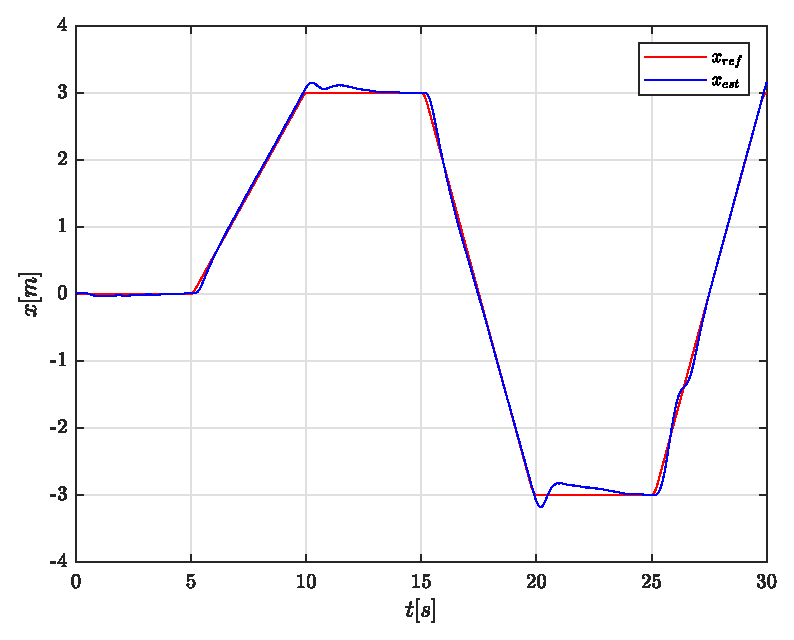
\includegraphics[width=1\textwidth]{Simulazioni/Figure/SMC/BUTTERFLY/PositionControlXPos}
		\caption{Controllo posizione lungo x}
		\label{fig:BUTTERFLYerrposxSMC}
	\end{subfigure}
	\hfill
	\begin{subfigure}{0.45\textwidth}
		\centering
		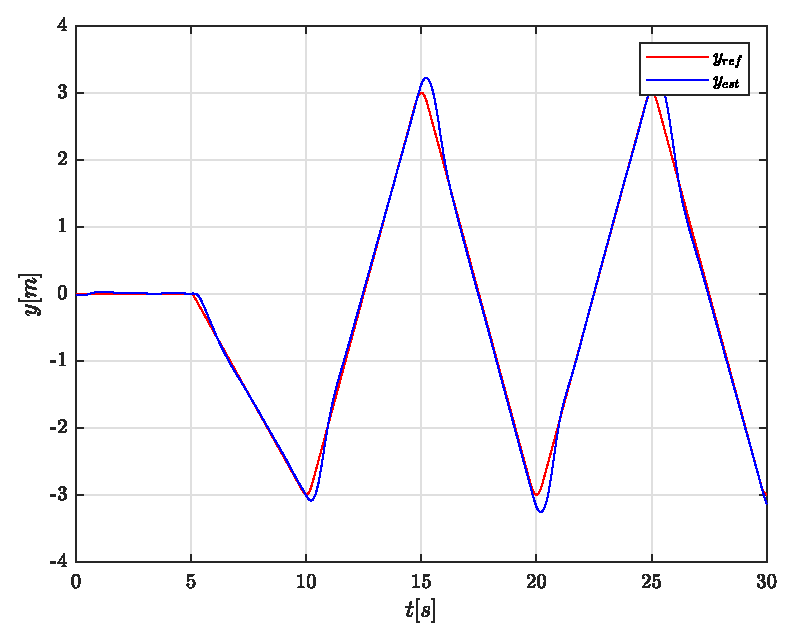
\includegraphics[width=1\textwidth]{Simulazioni/Figure/SMC/BUTTERFLY/PositionControlYPos}
		\caption{Controllo posizione lungo y}
		\label{fig:BUTTERFLYerrposySMC}
	\end{subfigure}
	\caption{Risposta in posizione con controllore SMC al comando BUTTERFLY}
\end{figure}

\begin{figure}
	\centering
	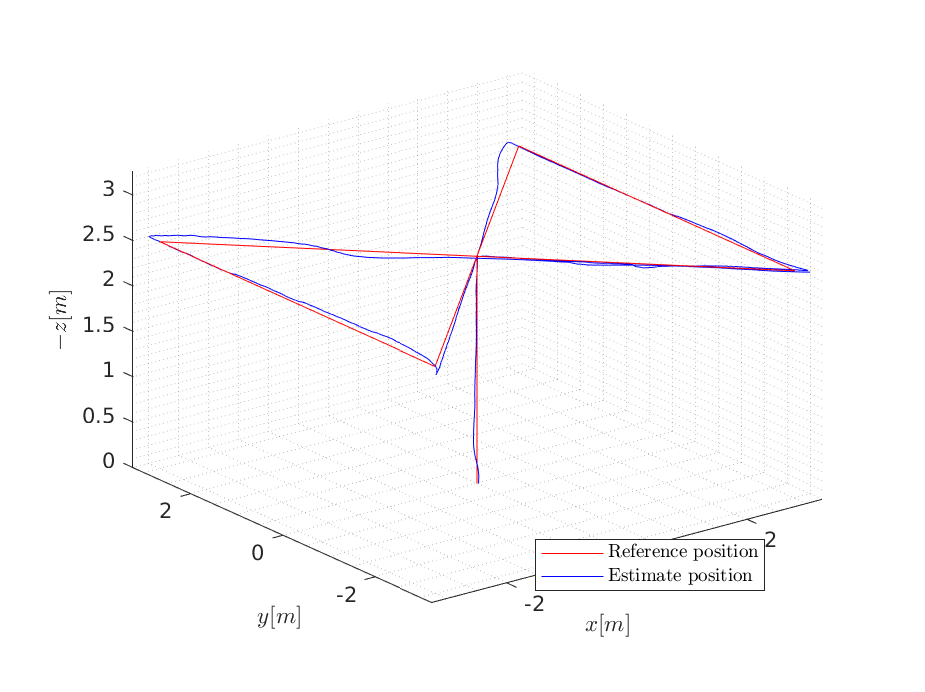
\includegraphics[width=0.65\textwidth]{Simulazioni/Figure/SMC/BUTTERFLY/Trajectory}
	\caption{Traiettoria percorsa con controllore SMC al segnale BUTTERFLY}
	\label{fig:BUTTERFLYtraSMC}
\end{figure}

\begin{figure}
	\centering
	\begin{subfigure}{0.45\textwidth}
		\centering
		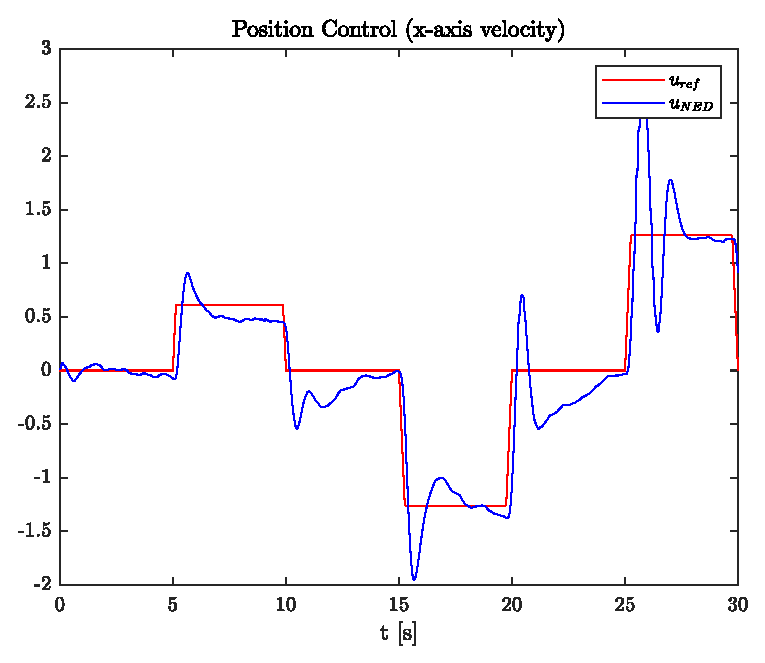
\includegraphics[width=1\textwidth]{Simulazioni/Figure/SMC/BUTTERFLY/PositionControlXVel}
		\caption{Controllo velocità lungo x}
		\label{fig:BUTTERFLYerrvelxSMC}
	\end{subfigure}
	\hfill
	\begin{subfigure}{0.45\textwidth}
		\centering
		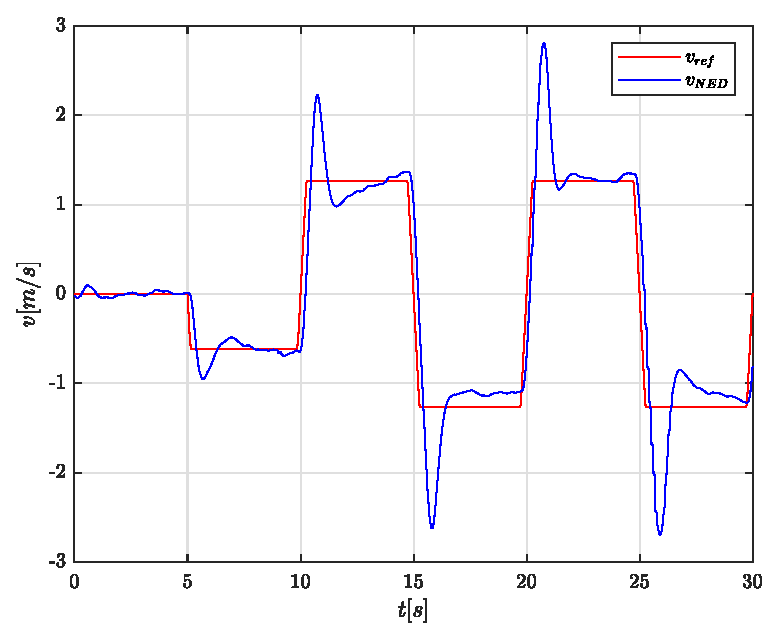
\includegraphics[width=1\textwidth]{Simulazioni/Figure/SMC/BUTTERFLY/PositionControlYVel}
		\caption{Controllo velocità lungo y}
		\label{fig:BUTTERFLYerrvelySMC}
	\end{subfigure}
	\caption{Risposta in velocità con controllore SMC al comando BUTTERFLY}
\end{figure}

\begin{figure}
	\centering
	\begin{subfigure}{0.45\textwidth}
		\centering
		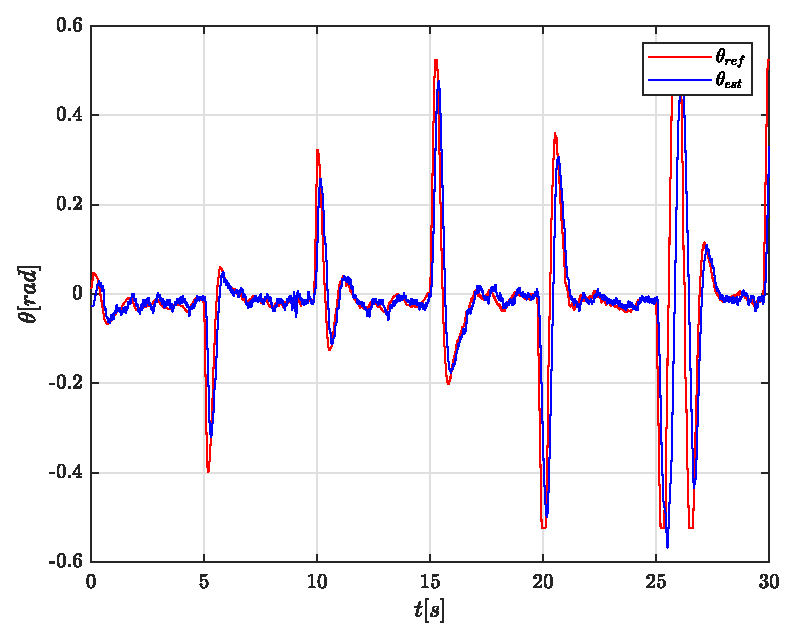
\includegraphics[width=1\textwidth]{Simulazioni/Figure/SMC/BUTTERFLY/AttitudeControlPitch}
		\caption{Controllo beccheggio}
		\label{fig:BUTTERFLYbecSMC}
	\end{subfigure}
	\hfill
	\begin{subfigure}{0.45\textwidth}
		\centering
		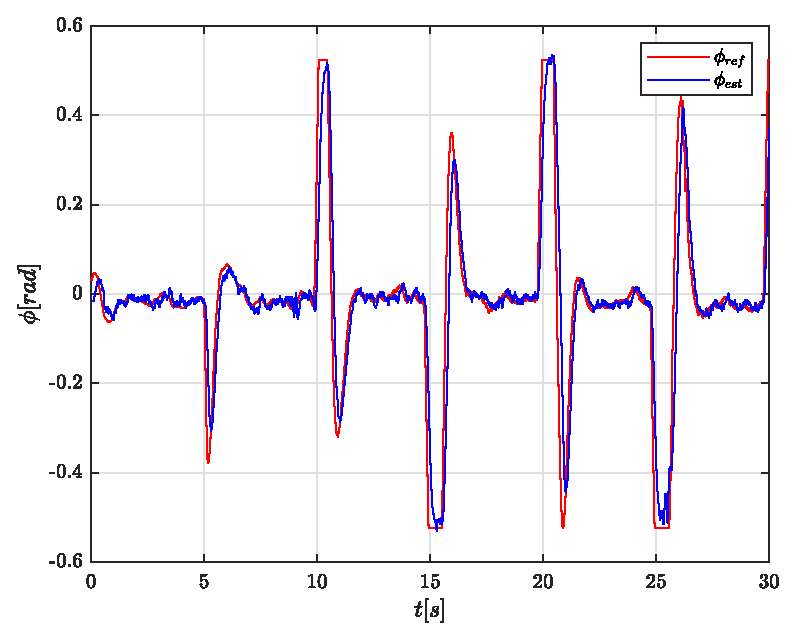
\includegraphics[width=1\textwidth]{Simulazioni/Figure/SMC/BUTTERFLY/AttitudeControlRoll}
		\caption{Controllo rollio}
		\label{fig:BUTTERFLYrolSMC}
	\end{subfigure}
	\hfill
	\begin{subfigure}{0.45\textwidth}
		\centering
		\includegraphics[width=1\textwidth]{Simulazioni/Figure/SMC/BUTTERFLY/AttitudeControlYaw}
		\caption{Controllo imbardata}
		\label{fig:BUTTERFLYyawSMC}
	\end{subfigure}
	\caption{Risposta dell' assetto con controllore SMC al comando BUTTERFLY}
\end{figure}

\begin{figure}
	\centering
	\includegraphics[width=0.45\textwidth]{Simulazioni/Figure/SMC/BUTTERFLY/PWM}
	\caption{Segnali PWM del controllore SMC al segnale BUTTERFLY}
	\label{fig:BUTTERFLYPWMSMC}
\end{figure}

Nella seguente simulazione l'andamento è simile al precedente caso, la posizione di riferimento è seguita con precisione nonostante la maggiore variazione di direzione, Figure (\ref{fig:BUTTERFLYerrposxSMC}) e (\ref{fig:BUTTERFLYerrposySMC}). Nella parte finale della simulazione, a circa 25 secondi dall'inizio della prova, Figura (\ref{fig:BUTTERFLYerrposxSMC}), si  osserva l'innesco di un modo oscillatorio smorzato dovuto probabilmente all'accoppiamento della dinamica con la variazione di direzione e il rumore di misurazione introdotta dai sensori. Questo effetto è osservabile anche in Figura (\ref{fig:BUTTERFLYerrvelxSMC}). L'inseguimento del profilo di velocità è comunque rispettato correttamento presentatno solo dei piccoli overshoot nella fase di variazione maggiore di velocità, Figure (\ref{fig:BUTTERFLYerrvelxSMC}) e (\ref{fig:BUTTERFLYerrvelySMC}). Anche in questo caso l'andamento del segnale di riferimento generato dal Position Controller è simile al precedente, Figure (\ref{fig:BUTTERFLYbecSMC}) e (\ref{fig:BUTTERFLYrolSMC}). In prossimità dell'oscillazione citata precedentemente, si osserva una maggiore saturazione del segnale di riferimento, nonostante ciò la risposta e stabile e precisa, Figura(\ref{fig:BUTTERFLYbecSMC}). Il segnale PWM , Figura (\ref{fig:BUTTERFLYPWMSMC}), presenta il tipico andamento discontinuo come nelle simulazioni precedenti. Si nota nella fase terminale della simulazione, l'incremento di questa oscillazione dovuto al controllo effettuato per correggere il modo che si è innescato a 25 secondi.

L'ultima missione riguarda la missione più completa denominata SNAKE, descritta in dettaglio nella sezione precedente.

\begin{figure}
	\centering
	\begin{subfigure}{0.45\textwidth}
		\centering
		\includegraphics[width=1\textwidth]{Simulazioni/Figure/SMC/SNAKE/PositionControlXPos}
		\caption{Controllo posizione lungo x}
		\label{fig:SNAKEerrposxSMC}
	\end{subfigure}
	\hfill
	\begin{subfigure}{0.45\textwidth}
		\centering
		\includegraphics[width=1\textwidth]{Simulazioni/Figure/SMC/SNAKE/PositionControlYPos}
		\caption{Controllo posizione lungo y}
		\label{fig:SNAKEerrposySMC}
	\end{subfigure}
	\caption{Risposta in posizione con controllore SMC al comando SNAKE}
\end{figure}

\begin{figure}
	\centering
	\includegraphics[width=0.65\textwidth]{Simulazioni/Figure/SMC/SNAKE/Trajectory}
	\caption{Traiettoria percorsa con controllore SMC al segnale SNAKE}
	\label{fig:SNAKEtraSMC}
\end{figure}

\begin{figure}
	\centering
	\begin{subfigure}{0.45\textwidth}
		\centering
		\includegraphics[width=1\textwidth]{Simulazioni/Figure/SMC/SNAKE/PositionControlXVel}
		\caption{Controllo velocità lungo x}
		\label{fig:SNAKEerrvelxSMC}
	\end{subfigure}
	\hfill
	\begin{subfigure}{0.45\textwidth}
		\centering
		\includegraphics[width=1\textwidth]{Simulazioni/Figure/SMC/SNAKE/PositionControlYVel}
		\caption{Controllo velocità lungo y}
		\label{fig:SNAKEerrvelySMC}
	\end{subfigure}
	\caption{Risposta in velocità con controllore SMC al comando SNAKE}
\end{figure}

\begin{figure}
	\centering
	\begin{subfigure}{0.45\textwidth}
		\centering
		\includegraphics[width=1\textwidth]{Simulazioni/Figure/SMC/SNAKE/AttitudeControlPitch}
		\caption{Controllo beccheggio}
		\label{fig:SNAKEbecSMC}
	\end{subfigure}
	\hfill
	\begin{subfigure}{0.45\textwidth}
		\centering
		\includegraphics[width=1\textwidth]{Simulazioni/Figure/SMC/SNAKE/AttitudeControlRoll}
		\caption{Controllo rollio}
		\label{fig:SNAKErolSMC}
	\end{subfigure}
	\hfill
	\begin{subfigure}{0.45\textwidth}
		\centering
		\includegraphics[width=1\textwidth]{Simulazioni/Figure/SMC/SNAKE/AttitudeControlYaw}
		\caption{Controllo imbardata}
		\label{fig:SNAKEyawSMC}
	\end{subfigure}
	\caption{Risposta dell' assetto con controllore SMC al comando SNAKE}
\end{figure}


\begin{figure}
	\centering
	\includegraphics[width=0.45\textwidth]{Simulazioni/Figure/SMC/SNAKE/PWM}
	\caption{Segnali PWM del controllore SMC al segnale SNAKE}
	\label{fig:SNAKEPWMSMC}
\end{figure}

In questa simulazione più lunga, non si presentano particolari moti oscillatori come nella precedente. La risposta in termini di posizioni è molto fedele al riferimento, con scostamenti solo in prossimità dei cambi di direzione, Figure (\ref{fig:SNAKEerrposxSMC}) e (\ref{fig:SNAKEerrposySMC}). Lo stesso discorso vale per il profilo di velocità. Sono visibili brevi tratti in cui si verifica overshoot e il successivo rapido assestamento mediamente sulla velocità di riferimento, Figure (\ref{fig:SNAKEerrvelxSMC}) e (\ref{fig:SNAKEerrvelySMC}). Nelle stesse Figure, nella fase terminale del volo, a circa 80 secondi dall'inizio di missione, durante la discesa, si può notare un incremento delle oscillazioni. Queste oscillazioni sono visibili anche nei restanti grafici relativi a questa simulazione. Analizzando la Figura (\ref{fig:SNAKEPWMSMC}), si osserva la presenza di alcuni tratti nella quale si presenta la saturazione del segnale ed un incremento considerevole della componente oscillatoria del segnale. Questa è ben visibile soprattutto nella parte finale del volo a circa 80 secondi dall'inizio della simulazione, in fase di discesa.

\subsection{Confronto}

\begin{figure}
	\centering
	\begin{subfigure}{0.48\textwidth}
		\centering
		\includegraphics[width=1\textwidth]{Simulazioni/Figure/Confronto/ERRPID}
		\caption{Controllore PID}
	\end{subfigure}
	\hfill
	\begin{subfigure}{0.48\textwidth}
		\centering
		\includegraphics[width=1\textwidth]{Simulazioni/Figure/Confronto/ERRSMC}
		\caption{ SMC}
	\end{subfigure}
	\caption{Errori di posizione tra PID e SMC nel tempo nelle simulazioni SIL}
	\label{fig:errori}
\end{figure}

Comparando le simulazioni sopra-riportate, si può affermare la superiorità di inseguimento del riferimento del controllore PID rispetto al controllore SMC. Nel controllore PID, il Position Controller genera un segnale in uscita molto discontinuo, a causa dell'amplificazione dell'errore di misurazione dovuto alla derivazione numerica calcolata sulla velocità. Come mostrato nella tesi \cite{DesTestCarm}, questa derivata però migliora la risposta di un semplice controllo proporzionale derivativo. Nel controllore SMC, la derivata della velocità non viene utilizzata e il coefficiente $K_{dd}$ è nullo. L'efficacia del Attitude Control con SMC però compensa appieno la perdita di precisione del Position Controller senza contributo derivativo, risultando complessivamente più preciso del controllore PID. D'altro canto il controllore PID, pur attuando una traiettoria meno precisamente rispetto al SMC, mostra una variazione di assetto meno rapido e più smorzato, anche a causa della linearità del comando PWM generato. Esso infatti è quasi privo di componente oscillante e di saturazione del comando, a differenza del comando PWM generato dal controllore SMC, che presenta una componente discontinua costante. Confrontando questo comportamento si può affermare che l'azionamento del controllore SMC è molto più aggressivo di quello del controllore PID, considerazione che si traduce in un consumo di batteria maggiore del controllore SMC.

Nella Tabella (\ref{tab:ConfrontoPIDSMCSIL}), vengono riportate scostamento massimo e medio sulla posizione calcolate con le formule (\ref{eq:err_max}) e (\ref{eq:err_med}), rispettivamente. Nella Figura (\ref{fig:errori}), viene mostrato l'andamento dell'errore nel tempo, nella quale è possibile valutare quantitativamente la migliore prestazione ottenuta dal controllore SMC rispetto al PID. Si nota dall'analisi dell'errore che il valore massimo in entrambi i casi viene misurato nella prima accelerazione, subito dopo il decollo, Figura (\ref{fig:errori}).

\begin{equation}\label{eq:err_max}
\epsilon_{max} = \max \sqrt{(x_{ref}-x_{est})^2+(y_{ref}-y_{est})^2+(z_{ref}-z_{est})^2}
\end{equation}

\begin{equation}\label{eq:err_med}
\epsilon_{medio} = \frac{1}{T_f}\int_{0}^{T_f} \sqrt{(x_{ref}-x_{est})^2+(y_{ref}-y_{est})^2+(z_{ref}-z_{est})^2} \ dt
\end{equation}

\begin{table}
	\centering
	\caption{Errori di posizione al comando SNAKE attraverso simulazione MIL}
	\begin{tabular}{c c c}
		\hline
		Errore &  PID [m] & SMC [m] \\
		\hline
		 $\epsilon_{max}$ & 0.37 & 0.29  \\
		 $\epsilon_{medio}$ & 0.08 & 0.03  \\
		\hline
	\end{tabular}	
	\label{tab:ConfrontoPIDSMCSIL}
\end{table}


